% Options for packages loaded elsewhere
\PassOptionsToPackage{unicode}{hyperref}
\PassOptionsToPackage{hyphens}{url}
\PassOptionsToPackage{dvipsnames,svgnames,x11names}{xcolor}
%
\documentclass[
  letterpaper,
  DIV=11,
  numbers=noendperiod]{scrartcl}

\usepackage{amsmath,amssymb}
\usepackage{iftex}
\ifPDFTeX
  \usepackage[T1]{fontenc}
  \usepackage[utf8]{inputenc}
  \usepackage{textcomp} % provide euro and other symbols
\else % if luatex or xetex
  \usepackage{unicode-math}
  \defaultfontfeatures{Scale=MatchLowercase}
  \defaultfontfeatures[\rmfamily]{Ligatures=TeX,Scale=1}
\fi
\usepackage{lmodern}
\ifPDFTeX\else  
    % xetex/luatex font selection
\fi
% Use upquote if available, for straight quotes in verbatim environments
\IfFileExists{upquote.sty}{\usepackage{upquote}}{}
\IfFileExists{microtype.sty}{% use microtype if available
  \usepackage[]{microtype}
  \UseMicrotypeSet[protrusion]{basicmath} % disable protrusion for tt fonts
}{}
\makeatletter
\@ifundefined{KOMAClassName}{% if non-KOMA class
  \IfFileExists{parskip.sty}{%
    \usepackage{parskip}
  }{% else
    \setlength{\parindent}{0pt}
    \setlength{\parskip}{6pt plus 2pt minus 1pt}}
}{% if KOMA class
  \KOMAoptions{parskip=half}}
\makeatother
\usepackage{xcolor}
\setlength{\emergencystretch}{3em} % prevent overfull lines
\setcounter{secnumdepth}{-\maxdimen} % remove section numbering
% Make \paragraph and \subparagraph free-standing
\ifx\paragraph\undefined\else
  \let\oldparagraph\paragraph
  \renewcommand{\paragraph}[1]{\oldparagraph{#1}\mbox{}}
\fi
\ifx\subparagraph\undefined\else
  \let\oldsubparagraph\subparagraph
  \renewcommand{\subparagraph}[1]{\oldsubparagraph{#1}\mbox{}}
\fi


\providecommand{\tightlist}{%
  \setlength{\itemsep}{0pt}\setlength{\parskip}{0pt}}\usepackage{longtable,booktabs,array}
\usepackage{calc} % for calculating minipage widths
% Correct order of tables after \paragraph or \subparagraph
\usepackage{etoolbox}
\makeatletter
\patchcmd\longtable{\par}{\if@noskipsec\mbox{}\fi\par}{}{}
\makeatother
% Allow footnotes in longtable head/foot
\IfFileExists{footnotehyper.sty}{\usepackage{footnotehyper}}{\usepackage{footnote}}
\makesavenoteenv{longtable}
\usepackage{graphicx}
\makeatletter
\def\maxwidth{\ifdim\Gin@nat@width>\linewidth\linewidth\else\Gin@nat@width\fi}
\def\maxheight{\ifdim\Gin@nat@height>\textheight\textheight\else\Gin@nat@height\fi}
\makeatother
% Scale images if necessary, so that they will not overflow the page
% margins by default, and it is still possible to overwrite the defaults
% using explicit options in \includegraphics[width, height, ...]{}
\setkeys{Gin}{width=\maxwidth,height=\maxheight,keepaspectratio}
% Set default figure placement to htbp
\makeatletter
\def\fps@figure{htbp}
\makeatother
% definitions for citeproc citations
\NewDocumentCommand\citeproctext{}{}
\NewDocumentCommand\citeproc{mm}{%
  \begingroup\def\citeproctext{#2}\cite{#1}\endgroup}
\makeatletter
 % allow citations to break across lines
 \let\@cite@ofmt\@firstofone
 % avoid brackets around text for \cite:
 \def\@biblabel#1{}
 \def\@cite#1#2{{#1\if@tempswa , #2\fi}}
\makeatother
\newlength{\cslhangindent}
\setlength{\cslhangindent}{1.5em}
\newlength{\csllabelwidth}
\setlength{\csllabelwidth}{3em}
\newenvironment{CSLReferences}[2] % #1 hanging-indent, #2 entry-spacing
 {\begin{list}{}{%
  \setlength{\itemindent}{0pt}
  \setlength{\leftmargin}{0pt}
  \setlength{\parsep}{0pt}
  % turn on hanging indent if param 1 is 1
  \ifodd #1
   \setlength{\leftmargin}{\cslhangindent}
   \setlength{\itemindent}{-1\cslhangindent}
  \fi
  % set entry spacing
  \setlength{\itemsep}{#2\baselineskip}}}
 {\end{list}}
\usepackage{calc}
\newcommand{\CSLBlock}[1]{\hfill\break\parbox[t]{\linewidth}{\strut\ignorespaces#1\strut}}
\newcommand{\CSLLeftMargin}[1]{\parbox[t]{\csllabelwidth}{\strut#1\strut}}
\newcommand{\CSLRightInline}[1]{\parbox[t]{\linewidth - \csllabelwidth}{\strut#1\strut}}
\newcommand{\CSLIndent}[1]{\hspace{\cslhangindent}#1}

\KOMAoption{captions}{tableheading}
\usepackage{lineno} \linenumbers
\makeatletter
\@ifpackageloaded{caption}{}{\usepackage{caption}}
\AtBeginDocument{%
\ifdefined\contentsname
  \renewcommand*\contentsname{Table of contents}
\else
  \newcommand\contentsname{Table of contents}
\fi
\ifdefined\listfigurename
  \renewcommand*\listfigurename{List of Figures}
\else
  \newcommand\listfigurename{List of Figures}
\fi
\ifdefined\listtablename
  \renewcommand*\listtablename{List of Tables}
\else
  \newcommand\listtablename{List of Tables}
\fi
\ifdefined\figurename
  \renewcommand*\figurename{Figure}
\else
  \newcommand\figurename{Figure}
\fi
\ifdefined\tablename
  \renewcommand*\tablename{Table}
\else
  \newcommand\tablename{Table}
\fi
}
\@ifpackageloaded{float}{}{\usepackage{float}}
\floatstyle{ruled}
\@ifundefined{c@chapter}{\newfloat{codelisting}{h}{lop}}{\newfloat{codelisting}{h}{lop}[chapter]}
\floatname{codelisting}{Listing}
\newcommand*\listoflistings{\listof{codelisting}{List of Listings}}
\makeatother
\makeatletter
\makeatother
\makeatletter
\@ifpackageloaded{caption}{}{\usepackage{caption}}
\@ifpackageloaded{subcaption}{}{\usepackage{subcaption}}
\makeatother
\ifLuaTeX
  \usepackage{selnolig}  % disable illegal ligatures
\fi
\usepackage{bookmark}

\IfFileExists{xurl.sty}{\usepackage{xurl}}{} % add URL line breaks if available
\urlstyle{same} % disable monospaced font for URLs
\hypersetup{
  pdftitle={Neural correlates of the deployment of spatial attention, and their modulation by repetitive movements},
  pdfauthor={Cameron Smith\^{}\{1\}; Daniel H. Baker\^{}\{1,2\}},
  colorlinks=true,
  linkcolor={blue},
  filecolor={Maroon},
  citecolor={Blue},
  urlcolor={Blue},
  pdfcreator={LaTeX via pandoc}}

\title{Neural correlates of the deployment of spatial attention, and
their modulation by repetitive movements}
\author{Cameron Smith\(^{1}\) \and Daniel H. Baker\(^{1,2}\)}
\date{}

\begin{document}
\maketitle

\(^1\)Department of Psychology, University of York, UK\\
\(^2\)Corresponding author, email: daniel.baker@york.ac.uk

\section{Abstract}\label{abstract}

The deployment of spatial attention generates distinct neural signatures
that can be detected at the scalp. Here, we use multivariate pattern
analysis of EEG data to decode the deployment of spatial attention, and
ask if this is modulated by repetitive movements. `Stimming' movements
(also known as repetitive stereotypies), are widely reported in autism,
but also present in some neurotypical individuals. Stimming has
historically been viewed as a problematic behaviour, but many
individuals claim that stimming benefits attention. We first validated
our paradigm (a Posner-style cueing design), demonstrating above-chance
classification of cue direction from around 300ms post-cue onset. We
then investigated whether stimming modulates decoding accuracy and task
performance. Our results, consisting of data primarily from neurotypical
participants, do not suggest that stimming has a negative impact on an
individual's ability to attend, unless the individual does not typically
engage in stimming behaviours. This suggests interventions aiming to
reduce stimming behaviours are not necessarily warranted and highlights
the need for further research into the potential benefits of stimming
specifically within the autistic population. Future research might also
consider the potential overlap between autistic stimming and the
fidgeting behaviours which are characteristic of ADHD, to help
understand the significant overlaps between the characteristics of the
two conditions.

\emph{Keywords}: attention; MVPA; stimming; EEG

\section{Introduction}\label{introduction}

The ability to orient and control the deployment of our attention to
spatial locations or features of our environment is essential to our
ability to perform tasks, focusing on relevant stimuli and disregarding
those that are unnecessary for the task at hand {[}1--3{]}. A classic
technique for studying the deployment of attention in space is the
Posner cueing paradigm, which demonstrates that it is possible for
attention to be deployed to spatial locations independently of eye
movements {[}4{]}.

Individuals with neurodevelopmental disorders such as attention deficit
hyperactivity disorder (ADHD) and autism present with deficits in
attention {[}5{]}. It has been suggested that repetitive stereotypies,
or `stimming' behaviours, are linked to these deficits in attention --
in the few studies where they have been asked, individuals who stim
report that it benefits their ability to focus, and that the behaviours
aid in emotional regulation {[}6--10{]}. It has been proposed that an
improved ability to focus through stimming may have a neural basis
{[}11{]}. Building on these theories and research, we tested the effect
of stimming on performance in a Posner cueing task.

The Posner cueing paradigm {[}4{]} involves the participant attending to
a central fixation point, then receiving a cue (which may be exogenous,
where attention is captured through bottom-up processes; or endogenous,
where attention is controlled by top-down processes, such as attending
selectively to cues of the correct colour {[}12{]}) indicating that a
stimulus is about to appear either to the left or the right of the
fixation point {[}13{]}. The assumption underlying the task is that if
participants successfully orient their attention to the cued location,
then their reaction times will be shorter and responses more accurate
for congruent trials (where the stimulus appears at the cued location)
than for incongruent trials (where the stimulus appears at the uncued
location); this has been demonstrated extensively {[}13{]}. The reaction
time difference was found by Posner {[}14{]} to be 25ms faster for
congruent trials and 40ms slower for incongruent trials, compared to a
neutral cue condition.

This paradigm has been combined with EEG to investigate the neural basis
of spatial attention. For example, Landau et al. {[}15{]} investigated
gamma-band activity during a Posner cueing task, comparing congruent and
incongruent trials. Gamma range responses were associated with voluntary
shifts in attention, e.g., attending to the left of the fixation point
following a left-pointing arrow cue, but were absent when attention was
involuntarily captured by the appearance of a stimulus in the uncued
location on incongruent trials; this suggests that voluntary and
involuntary processes of attention deployment are controlled by separate
mechanisms. Thiery et al. {[}13{]} investigated two specific ERPs, the
N2pc component (a negative response typically seen at around 200ms post
stimulus, in the posterior-contralateral region) and the SPCN component
(sustained posterior contralateral negativity). They used multivariate
pattern analysis and used the classifier accuracy to determine that
these two components were able to predict the focus of participants'
spatial attention. This was modulated by the varied distance of the
stimulus from the central fixation (further being better decoded).

A combined EEG and TMS study by Capotosto et al. {[}16{]} demonstrated
that the application of TMS to the right intraparietal sulcus (IPS)
impairs target detection, particularly on incongruent trials. They
additionally noted that the P3 response amplitude was affected by this;
on incongruent trials its amplitude was significantly lower, and on
congruent trials it was significantly higher. The IPS has been
previously identified as an important region in attentional deployment
by Vossel et al. {[}17{]} in an fMRI study identifying regions that are
selectively active on congruent and incongruent trials. The right IPS
and, additionally, the right inferior frontal gyrus were implicated in
attentional processes related to both types of trial. Peelen et al.
{[}18{]} concluded that both endogenous and exogenous orienting cues
involved the same network in their fMRI study, implicating frontal and
parietal regions (the premotor cortex, posterior parietal cortex, medial
frontal cortex, and right inferior frontal cortex). Fitzgerald et al.
{[}19{]} conducted an MRI study using the Posner cueing task and found
that activation in the ventral attention network differed between
individuals with autism and controls; individuals with autism also
showed weaker functional connectivity in the dorsal attentional network
compared to their neurotypical counterparts.

A number of developmental disorders involve deficits in attention,
notably ADHD and autism. In the case of ADHD, attention deficits are a
defining feature of the condition (American Psychological Association,
2013). For autism, attention deficits are not an explicit part of the
diagnostic criteria (although restricted interests, which are included,
are somewhat related), but both attentional deficits and strengths are
widely reported in autistic individuals. They are typically more
distractible, demonstrating `underselective' attention, but also
demonstrate `overselective' attention where they attend intensely to a
more limited subset of stimuli. This `overselective' attention has been
suggested to be linked to restricted interests, which is also sometimes
referred to as `hyperfocus', where a task is the subject of intense
focus for the individual {[}e.g., 20{]}. These differences appear to
have a neural basis -- they have been linked to unusually wide sulci in
the parietal lobe {[}5{]}. Hyperfocus is also widely self-reported in
ADHD, despite a lack of clinical research into the phenomenon {[}21{]}.

These marked differences in attentional deployment seen in both
conditions are worth considering in the framework of the transdiagnostic
approach, which seeks to identify core deficiencies that result in the
presentation of traits from multiple disorders, instead of approaching
different disorders as entirely separate even within the same individual
{[}22{]}. ADHD is the most common comorbidity of autism, and even
without a dual diagnosis, 30-80\% of individuals with autism present
symptoms of ADHD, and 20-60\% of children with ADHD exhibit autism-like
traits {[}23{]}. Some shared deficiencies that have already been
identified in the case of autism and ADHD include fine motor function
and verbal fluency, alongside some structural differences in the brain
{[}23{]}.

Stimming behaviours are commonly seen in individuals with diagnoses of
autism and/or ADHD, and involve repetitive movements, typically
featuring the arms, hands, or entire body {[}24{]}, for example hand
flapping {[}6{]}. They are also observed in neurotypical individuals,
but at much lower rates than in neurodiverse individuals {[}24{]}. The
behaviours are typically defined as involuntary, but pleasant
{[}6,7,24{]}, and are associated with emotional states such as stress,
boredom, concentration, or excitement {[}25{]}. They are often defined
as purposeless {[}e.g., 26{]} but self-reports from individuals with
autism claim that stimming aids the regulation of their emotions
{[}6,7{]} and concentration {[}8,10{]}.

A type of vocal stimming called echolalia has been consistently
demonstrated to have benefits for autistic children in the acquisition
of language {[}27,28{]}. This is one of the few instances that stimming
has been researched in terms of its potential function. Echolalic
utterances, which typically involve repeating words spoken by another,
have also been identified as having predominantly communicative
functions {[}29{]}. This opens up an avenue to research potential
benefits that other types of stimming may provide.

Current research into stimming is largely focussed on designing
interventions to eliminate the behaviours, for example the use of
weighted vests {[}30{]}. Taking this approach without first attempting
to understand if there are benefits to the behaviour seems ill-advised.
McCarty and Brumback {[}11{]}, for example, proposed based on
self-reports of the benefits of stimming (focus, coping with
overwhelming sensory input, and relaxation) that regular motor movements
may generate (or be a by-product of) rhythmic oscillations in the motor
cortex, which entrain oscillations in the sensory cortex. This
entrainment might improve information transfer in the sensory cortex,
effectively normalising the atypical motor and sensory oscillations
observed in the brains of autistic individuals both during tasks
{[}31--33{]} and at rest {[}34,35{]}.

There is heavy stigma around stimming behaviours, with many individuals
reporting they have been explicitly instructed not to stim, despite
attempts at repression causing them some discomfort {[}7{]}. Individuals
with autism state that they believe stimming should not be stigmatised
in this way, and that they should be allowed to act in the way that
feels natural to them {[}6{]}. They typically report that stimming is a
positive experience for them, and negative only when it is
self-injurious or stigmatized {[}9,36{]}, and there is a growing body of
evidence to suggest stimming has a communicative function {[}36,37{]}.
Research into potential benefits of stimming is important as a step
towards dispelling this stigma, and discouraging interventions that aim
to eliminate the behaviour.

This study involved two experiments. In the first experiment,
participants completed a Posner cueing task while EEG recordings were
taken; a pattern classifier then attempted to differentiate, using the
participants' brain activity, whether they attended to the left vs.~to
the right following the cue onset. This is similar to the methodology
used by Thiery et al. {[}13{]}: by measuring the timecourse of
classifier accuracy, we are provided with an index of the deployment of
spatial attention. The second experiment extended this paradigm by
adding a stimming condition. The accuracy of the classifier was compared
between conditions where the participants were permitted to stim during
the trials, or instructed to keep still. In this case, we used decoding
accuracy to assess whether stimming provided a benefit in terms of the
deployment of spatial attention; if there was a benefit, the classifier
accuracy would be higher, as the EEG signal would differ more between
conditions due to the greater focus of attention in different spatial
locations. For the purposes of our analyses, due to an insufficiently
sized and heterogeneous clinical group, we grouped the participants
based on whether or not they reported stimming in their everyday lives;
as discussed previously, neurotypicals often engage in stimming
{[}24{]}, and 64\% of our participants reported in the pre-experiment
questionnaire that they typically engaged in stimming.

\section{Methods}\label{methods}

\subsection{Participants}\label{participants}

41 participants took part in Experiment 1, but four produced very noisy
data so were excluded, leaving a sample of 37 participants (20 male, 17
female). A total of 22 participants took part in Experiment 2 (8 male,
14 female). Participants in Experiment 2 were asked to report diagnoses
of neurodevelopmental disorders -- 17 had no diagnosis, 2 had a
diagnosis of autism, and 3 had a diagnosis of ADHD. 15/22 participants
further reported they typically engaged in stimming behaviours, while 7
reported that they did not - this information was collected through a
single yes/no question asking if participants typically stim, due to a
lack of available self-report stimming scales. Both experiments were
granted ethical approval by the Ethics Committee of the Department of
Psychology at the University of York. The identification numbers were
356 for Experiment 1, and 173 for Experiment 2. Participants provided
written informed consent before data collection began. Data collection
for Experiment 1 began on 25th January 2017, and ended on 10th March
2017. Data collection for Experiment 2 began on 14th July 2022, and
ended on 14th September 2022.

\subsection{Apparatus and stimuli}\label{apparatus-and-stimuli}

Stimuli were displayed on a ViewPixx 3D display (VPixx Technologies
Inc., Quebec, Canada) with a diagonal extent of 24 inches, a refresh
rate of 120Hz, and a resolution of 1920x1080 pixels. The screen was
viewed by the participants from a distance of 57cm, resulting in a
spatial resolution of 36 pixels per degree of visual angle. The display
was gamma corrected using a Minolta LS110 photometer to ensure a linear
luminance response. Stimuli were generated and displayed using a Mac Pro
computer running Matlab, with the experiment script making use of
functions from Psychtoolbox 3 {[}38--40{]}.

In both experiments, EEG recordings were acquired using an ANT Neuroscan
64-channel EEG system (ANT Neuro, Hengelo, Netherlands). Electrodes were
mounted in a waveguard cap, arranged according to the 10/20 system, and
were referenced to the whole head average. The ground electrode was
located at position \emph{AFz}, and EEG signals were recorded at 1kHz.
In Experiment 2, participants' eye movements were also recorded using an
EyeLink 1000 (SR Research Ltd., Ottawa, Canada) eye tracker, also
sampling at 1kHz. Low-latency digital triggers were sent from the
stimulus computer to the EEG system using an 8-bit parallel cable.

Target stimuli in both experiments were horizontal sine-wave gratings
with a diameter of 4 degrees, and a spatial frequency of 2c/deg. The
target appeared offset by 8 degrees to either the left or the right of
the central fixation point. The base contrast of the target was 50\%,
and either the upper or lower half of the grating contained a contrast
increment of a further 10\%. Participants were asked to indicate whether
the upper or lower half of the grating contained the increment using
arrow keys on the computer keyboard. The fixation cross was 0.25
\(\times\) 0.25 degrees, and was displayed throughout.

Each trial was preceded by a cue. In Experiment 1 the cue was a face
with eyes pointing left or right. In Experiment 2 the cue was an arrow
pointing left or right. The face cues used in Experiment 1 were the
average of 22 female faces taken from the NimStim database {[}41{]} and
were digitally altered so that the eyes were directed to the left or the
right. The face had a width of 3 degrees and a height of 4 degrees and
was displayed in the centre of the screen. The arrow cue used in
Experiment 2 was 1.4 degrees long and was displayed in the centre of the
screen.

\subsection{Procedure}\label{procedure}

Participants in both experiments completed four blocks of the Posner
cueing task, with each block consisting of 200 trials. They were
instructed to keep their eyes focused on the central fixation cross, and
to attend to the gratings without shifting their gaze. During each
trial, participants viewed a fixation cross, which remained on the
screen throughout the trial (excluding times when the cue appeared on
the screen). The cue stimulus appeared for 200ms, followed by a randomly
determined gap of 400-600ms before the grating appeared on the screen.
The target grating was then displayed for 200ms. Participants were
required to report whether the upper or lower half of the grating
appeared higher in contrast; following their response, a randomly
determined interval drawn from a normal distribution (average 1000ms,
with a standard deviation of ±200ms) preceded the next appearance of the
cue. This procedure is illustrated in Figure~\ref{fig-methodsfig} for
the face cue (panel a) and the arrow cue (panel b). Cue congruence was
75\% in both experiments, meaning that each participant contributed a
total of 600 congruent trials and 200 incongruent trials across the
experiment.

\begin{figure}

\centering{

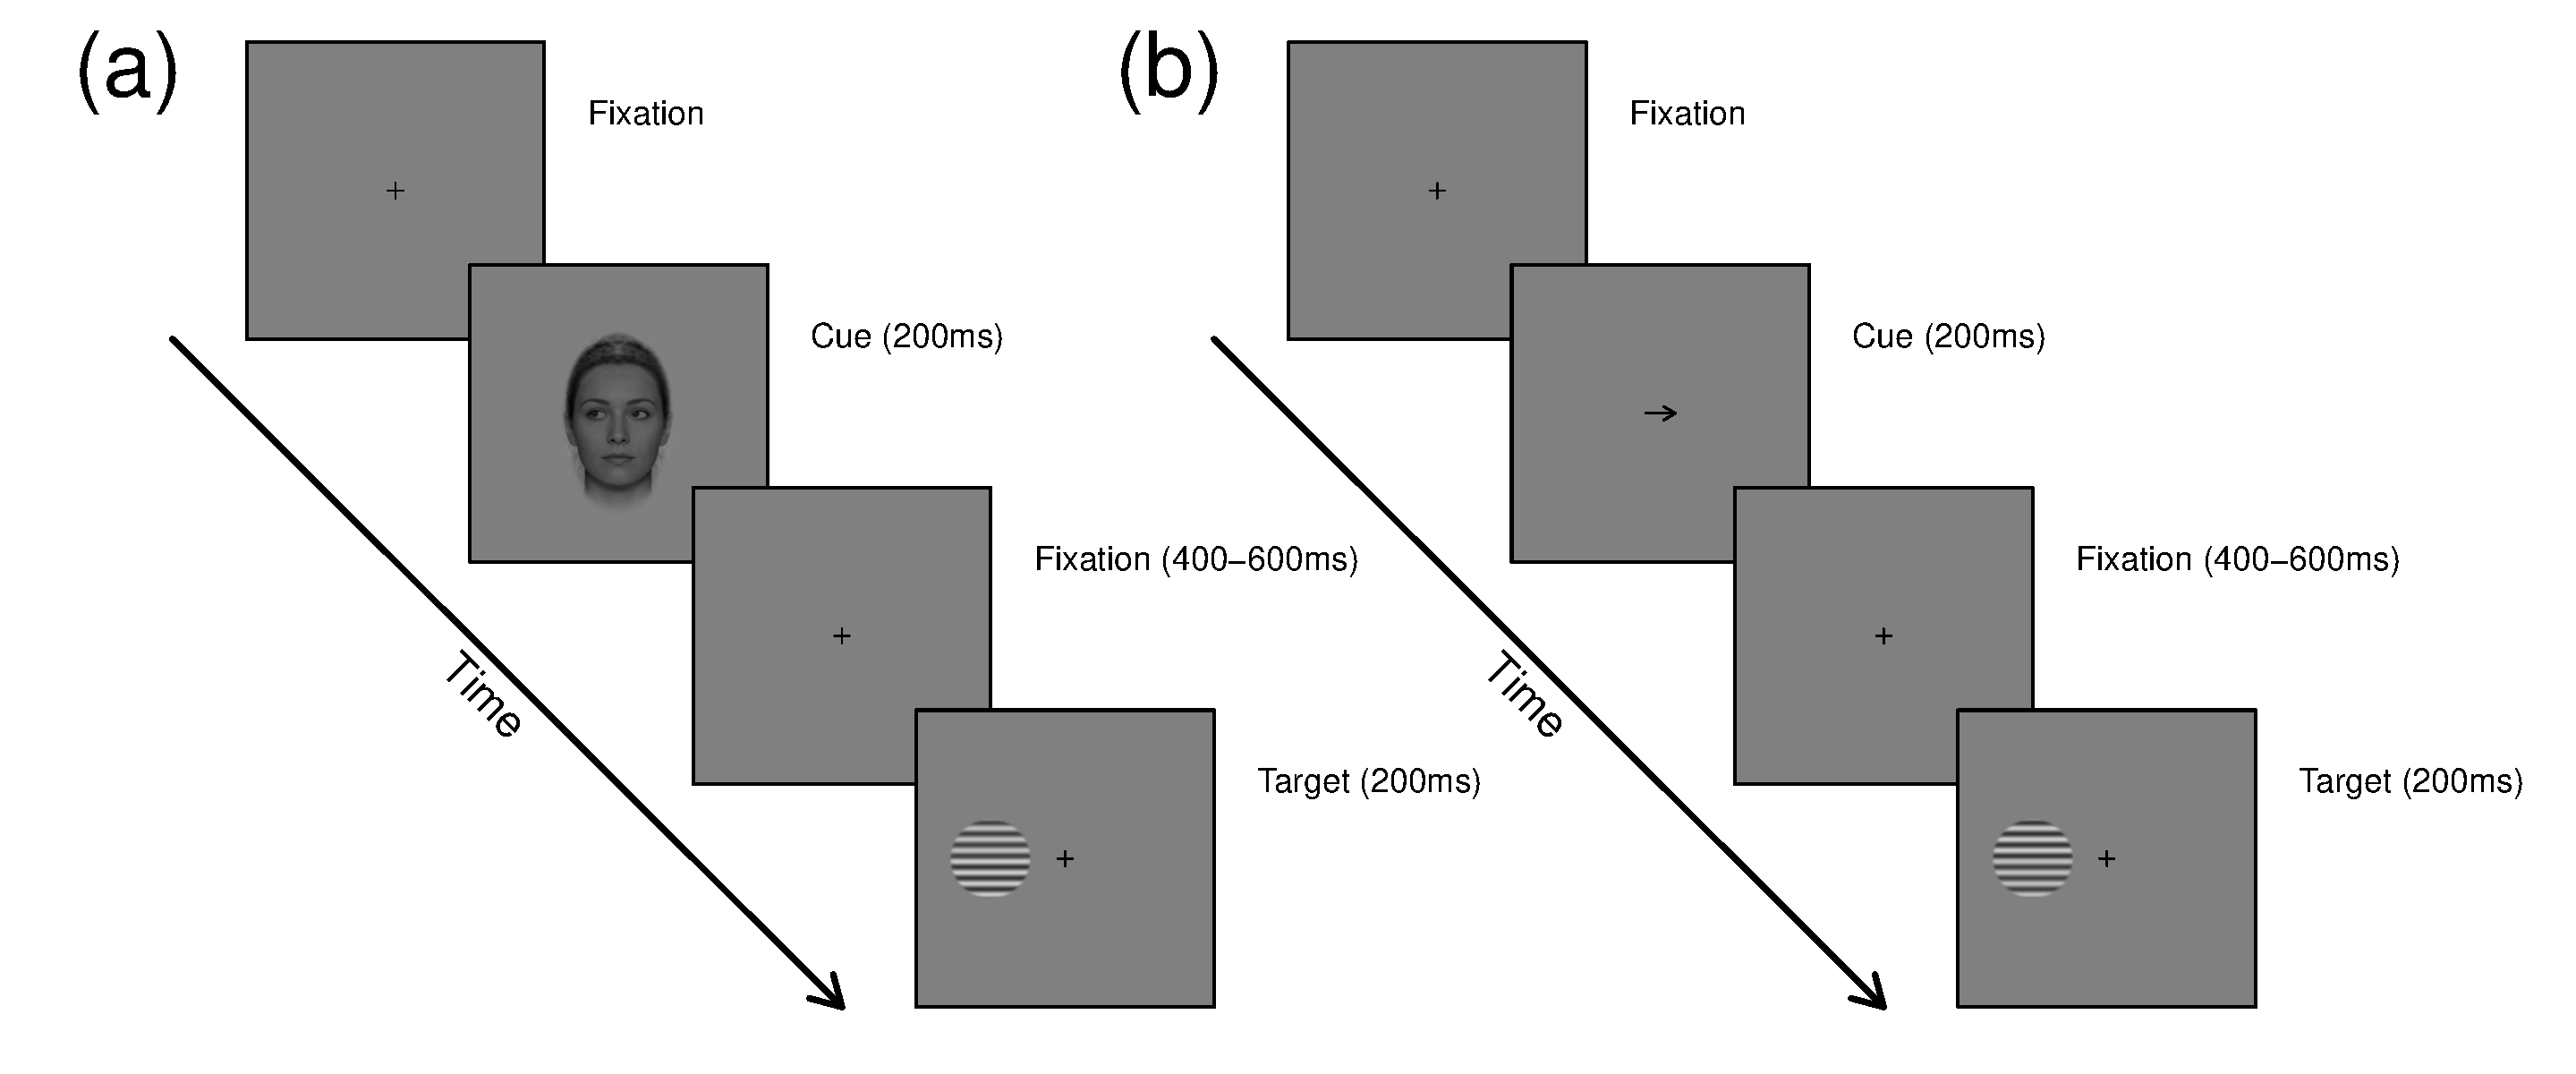
\includegraphics[width=0.95\textwidth,height=\textheight]{Figures/MethodsFigure.pdf}

}

\caption{\label{fig-methodsfig}Illustration of trial procedure for both
experiments. In panel (a), the cue was a face with eyes pointing to
either the left (as pictured) or the right. In panel (b), the cue was an
arrow. Target gratings had a contrast of 50\%, plus a 10\% increment in
either the upper or lower half. Note that images are not drawn to scale
in this schematic to aid visibility - see text for actual dimensions.}

\end{figure}%

In Experiment 2, participants were additionally instructed to stim,
using a movement restricted to one hand only, in half of the blocks.
This was to ensure minimal distortion of the EEG signal resulting from
movement. The order in which participants completed stimming or
non-stimming blocks was counterbalanced; half the participants were
instructed to stim on blocks 1 and 3, while the other half were
instructed to stim on blocks 2 and 4.

\subsection{Data analysis}\label{data-analysis}

Raw EEG data were converted into EEGlab .set format using Matlab and the
EEGlab toolbox {[}42{]}. We then used MNE python {[}43{]} for the main
analysis. Data were bandpass filtered between 0.2 and 30Hz, and then
epoched using the event timestamps. We performed classification using a
linear classifier with 10-fold cross-validation on the voltage data
across all electrodes (excluding electrodes \emph{M1} and \emph{M2}),
independently at each time point and for each participant. We then
averaged classification accuracy across participants to generate the
timecourses used in the main analysis. We calculate Bayes factors
{[}44{]} to compare classification accuracy to chance performance (50\%
correct) and to make comparisons between conditions and groups, but also
report frequentist tests for reference. We express Bayes factors in
logarithmic units to account for extreme values (\(log_{10}BF_{10}\)),
such that a Bayes factor of 3 is a \(log_{10}BF_{10}\) = 0.48, and
constitutes convincing evidence for the alternative hypothesis, a Bayes
factor of 10 is a \(log_{10}BF_{10}\) = 1, and constitutes strong
evidence for the alternative hypothesis, and a Bayes factor of 30 is a
\(log_{10}BF_{10}\) = 1.48, and constitutes overwhelming evidence for
the alternative hypothesis.

\subsection{Data and code
availability}\label{data-and-code-availability}

Raw data, processed data, and analysis scripts are freely available
through the project repository at: http://doi.org/10.17605/OSF.IO/YUHZ4.

\section{Results}\label{results}

\subsection{Experiment 1}\label{experiment-1}

We first analysed the behavioural responses from the experiment,
comparing accuracy and reaction times between stimuli shown in the cued
(i.e.~a congruent target) and uncued (an incongruent target) location.
There was a highly significant effect of cue congruency on both accuracy
(\(log_{10}BF_{10}\) = 1.77, \emph{t} = 3.82, \emph{p} \textless0.001,
\emph{d} = 0.61) and reaction time (\(log_{10}BF_{10}\) = 6.08, \emph{t}
= -7.26, \emph{p} \textless0.001, \emph{d} = 1.16), as shown in
Figure~\ref{fig-Expt1resps}. Responses to targets in the cued location
were both faster (\(M_{diff}\) = 51 ms) and more accurate (\(M_{diff}\)
= 3\%) than for those in the uncued location, showing a classic Posner
cueing effect.

\begin{figure}

\centering{

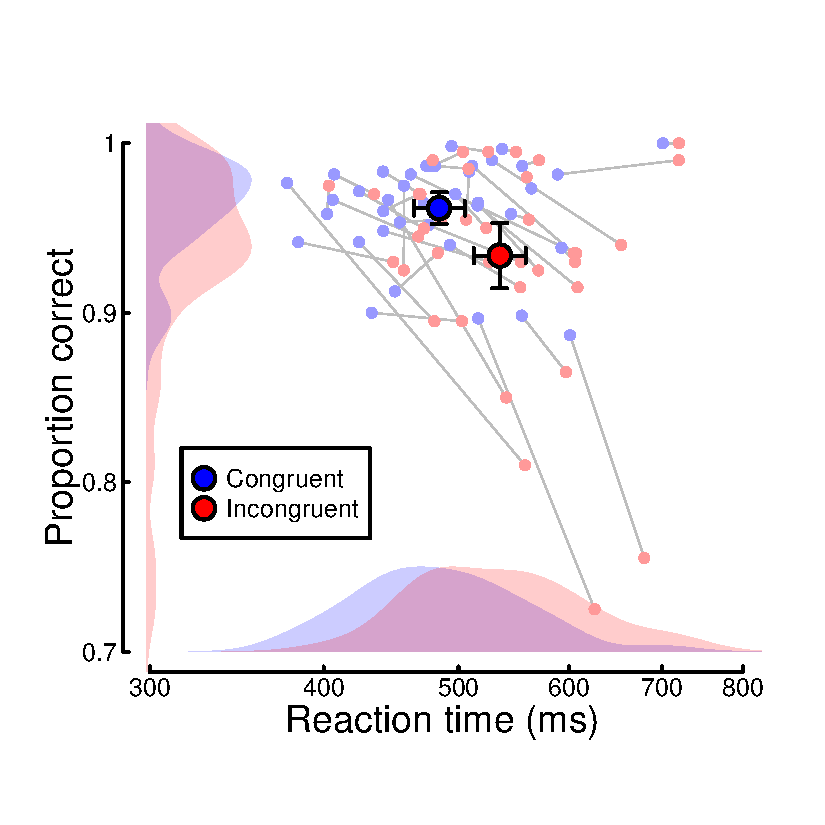
\includegraphics[width=0.6\textwidth,height=\textheight]{Figures/Exp1resps.pdf}

}

\caption{\label{fig-Expt1resps}Summary of reaction time and accuracy
data for the cueing task in Experiment 1. Small points show data for
individual participants (N = 39), and larger points give the group
means. Error bars indicate 95\% confidence intervals.}

\end{figure}%

We next explored the EEG data in response to both the cue presentation
and the target presentation. There were typical evoked potentials in
response to both types of stimulus, as summarised in
Figure~\ref{fig-Expt1EEG}b,c,e,f.~Patterns of voltage across the scalp
showed similar lateralisation effects both for cues pointing to either
the left or right, and for targets presented to either the left or
right. Multivariate pattern analysis was able to decode the side of cue
presentation from around 300ms after cue onset (see
Figure~\ref{fig-Expt1EEG}a), with a maximum accuracy of 69\%, and a
plateau of high performance from around 500-1000ms. This relatively late
onset of above-chance classification likely reflects the deployment of
covert spatial attention to one side of the visual field, and is
therefore a neural index of attentional focus. The pattern classifier
could decode the side of target presentation with much greater accuracy
(maximum of 89\%), from around 100ms after target onset (black curve in
Figure~\ref{fig-Expt1EEG}d). Finally, we were able to decode cue
congruency (i.e.~whether the target presented was on the side indicated
by the cue) with a maximum accuracy of 62\%, and a similar timecourse to
the decoding of target side (green curve in Figure~\ref{fig-Expt1EEG}d).
Overall, these results indicate that our EEG data are sufficiently
sensitive to provide an index of the deployment of spatial attention.

\begin{figure}

\centering{

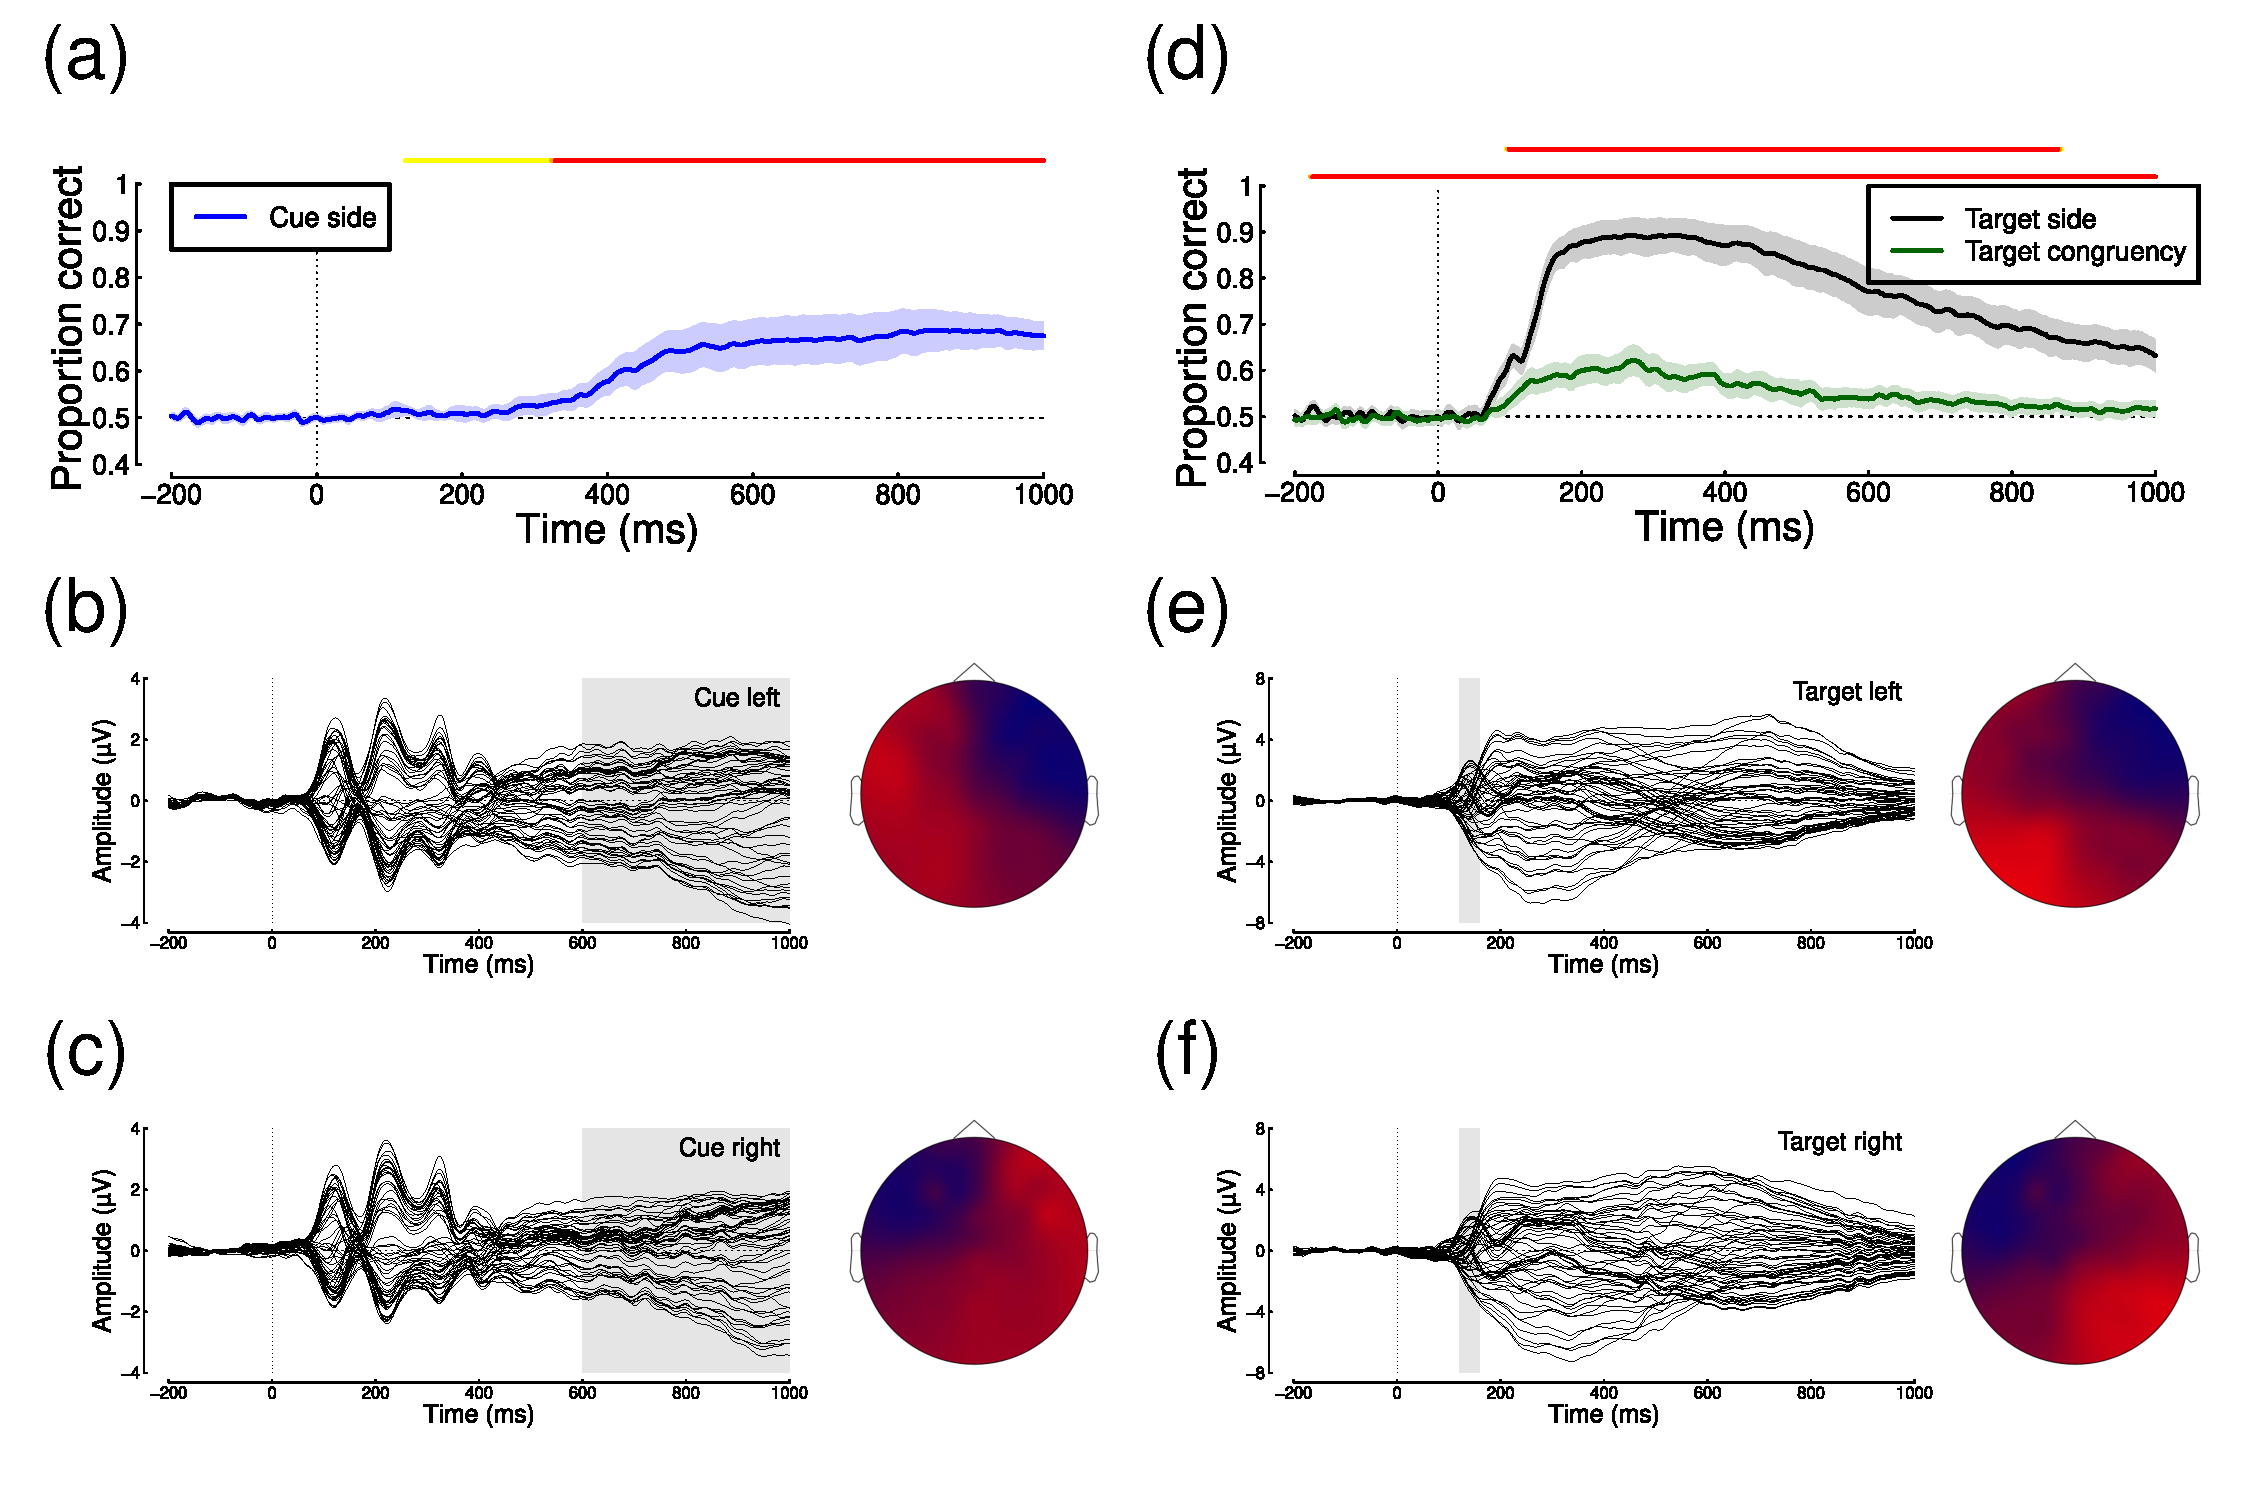
\includegraphics{Figures/Exp1summary.pdf}

}

\caption{\label{fig-Expt1EEG}Summary of EEG data from Experiment 1.
Panel (a) shows decoding accuracy of a pattern classification algorithm
trained on responses to the cue stimulus (Time 0 is the cue onset). ERPs
and scalp topographies are shown for cues pointing left (b) and right
(c), with the shaded regions indicating the time period over which
voltages were averaged to generate the scalp plots. Panel (d) shows
decoding accuracy for classifying target location (black curve) or cue
congruency (green curve) in response to the target (Time 0 is the target
onset). ERPs and scalp topographies are shown for targets on the left
(e) and right (f) side of fixation, with the shaded regions indicating
the time period over which voltages were averaged to generate the scalp
plots. Shaded regions in panels (a,d) indicate 95\% confidence
intervals, and lines above y=1 indicate Bayes factor scores above 3
(yellow \textgreater3; orange \textgreater10; red \textgreater30).}

\end{figure}%

\subsection{Experiment 2}\label{experiment-2}

In Experiment 2, we replicated the basic design of Experiment 1, but
this time with an added `stimming' condition, and with participants
divided into groups based on their self-reported stimming behaviour. The
results are summarised in Figure~\ref{fig-Expt2resps}. Pooling across
all participants, for response accuracy there was no effect of cue
congruency (\(log_{10}BF_{10}\) = -0.65, \emph{F} = 0.06, \emph{p} =
0.803, \(\eta^2_G\) = 0), stimming condition (\(log_{10}BF_{10}\) =
-0.66, \emph{F} = 0, \emph{p} = 0.977, \(\eta^2_G\) = 0), nor an
interaction between the two (\(log_{10}BF_{10}\) = -0.48, \emph{F} =
0.8, \emph{p} = 0.383, \(\eta^2_G\) = 0). For reaction time, there were
significant effects of cue congruency (\(log_{10}BF_{10}\) = 3.1,
\emph{F} = 29.28, \emph{p} \textless0.001, \(\eta^2_G\) = 0.07) and
stimming condition (\(log_{10}BF_{10}\) = 1.08, \emph{F} = 7.1, \emph{p}
= 0.01, \(\eta^2_G\) = 0.04), as well as an interaction between the two
(\(log_{10}BF_{10}\) = -0.34, \emph{F} = 12.03, \emph{p} = 0.002,
\(\eta^2_G\) = 0.01). Note that reactions were faster in the
non-stimming condition (591 ms) than in the stimming condition (632 ms).
These effects remained significant in the group who reported stimming in
their daily lives (N=14) for the effects of cue congruency
(\(log_{10}BF_{10}\) = 1.48, \emph{F} = 11.42, \emph{p} \textless{}
0.005, \(\eta^2_G\) = 0.06), stimming condition (\(log_{10}BF_{10}\) =
0.42, \emph{F} = 4.89, \emph{p} = 0.045, \(\eta^2_G\) = 0.03), and their
interaction (\(log_{10}BF_{10}\) = -0.33, \emph{F} = 8.71, \emph{p} =
0.011, \(\eta^2_G\) = 0.01). For the group who did not report stimming
(N=8), only the effect of cue congruency was significant
(\(log_{10}BF_{10}\) = 0.92, \emph{F} = 40.15, \emph{p} \textless0.001,
\(\eta^2_G\) = 0.11).

\begin{figure}

\centering{

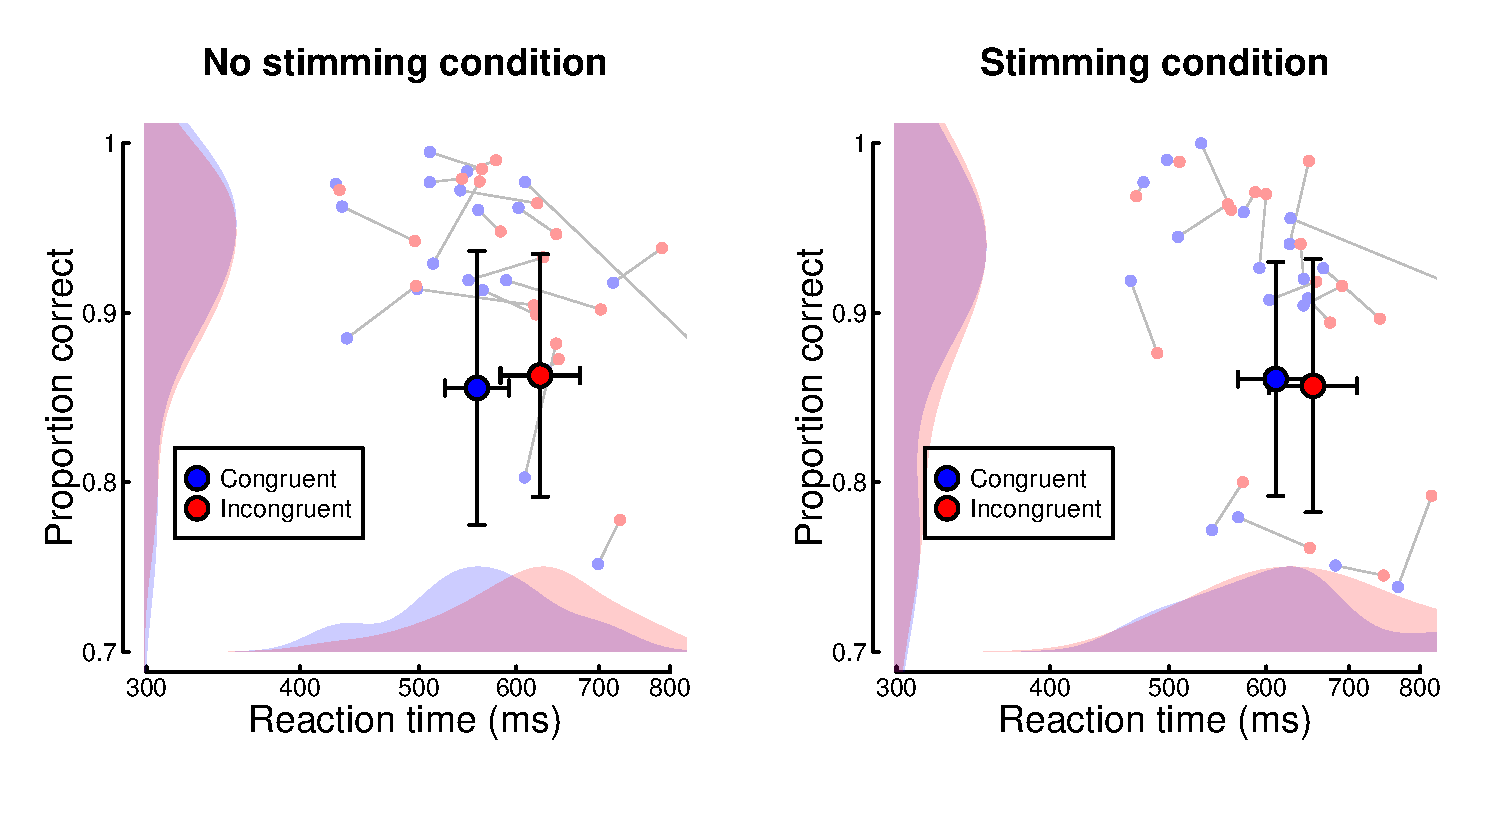
\includegraphics[width=0.95\textwidth,height=\textheight]{Figures/Exp2resps.pdf}

}

\caption{\label{fig-Expt2resps}Summary of reaction time and accuracy
data for the cueing task in Experiment 2. Small points show data for
individual participants (N = 22), and larger points give the group
means. Error bars indicate 95\% confidence intervals.}

\end{figure}%

The EEG results from Experiment 2 are summarised in
Figure~\ref{fig-Expt2EEG}. Panels (a,b) demonstrate that multivariate
pattern analysis is able to decode cue direction, target side, and
target congruency with similar timecourses to Experiment 1 (see
Figure~\ref{fig-Expt1EEG}), though with somewhat lower accuracy overall.
We then compared decoding accuracy for cue side and cue congruency
between the stimming group (N=14), and the non-stimming group (N=8).
Although decoding accuracy appeared to be slightly higher for the
non-stimming group for cue side (Figure~\ref{fig-Expt2EEG}c), this
difference was not convincing. Accuracy for cue congruency was very
similar for the two groups (Figure~\ref{fig-Expt2EEG}d). Finally, we
compared the deployment of spatial attention between stimming and
non-stimming conditions for each of the two groups. There appeared to be
a slight decrease in decoding accuracy in the non-stimming group when
they were asked to stim (Figure~\ref{fig-Expt2EEG}f), but no differences
in the stimming group (Figure~\ref{fig-Expt2EEG}e).

\begin{figure}

\centering{

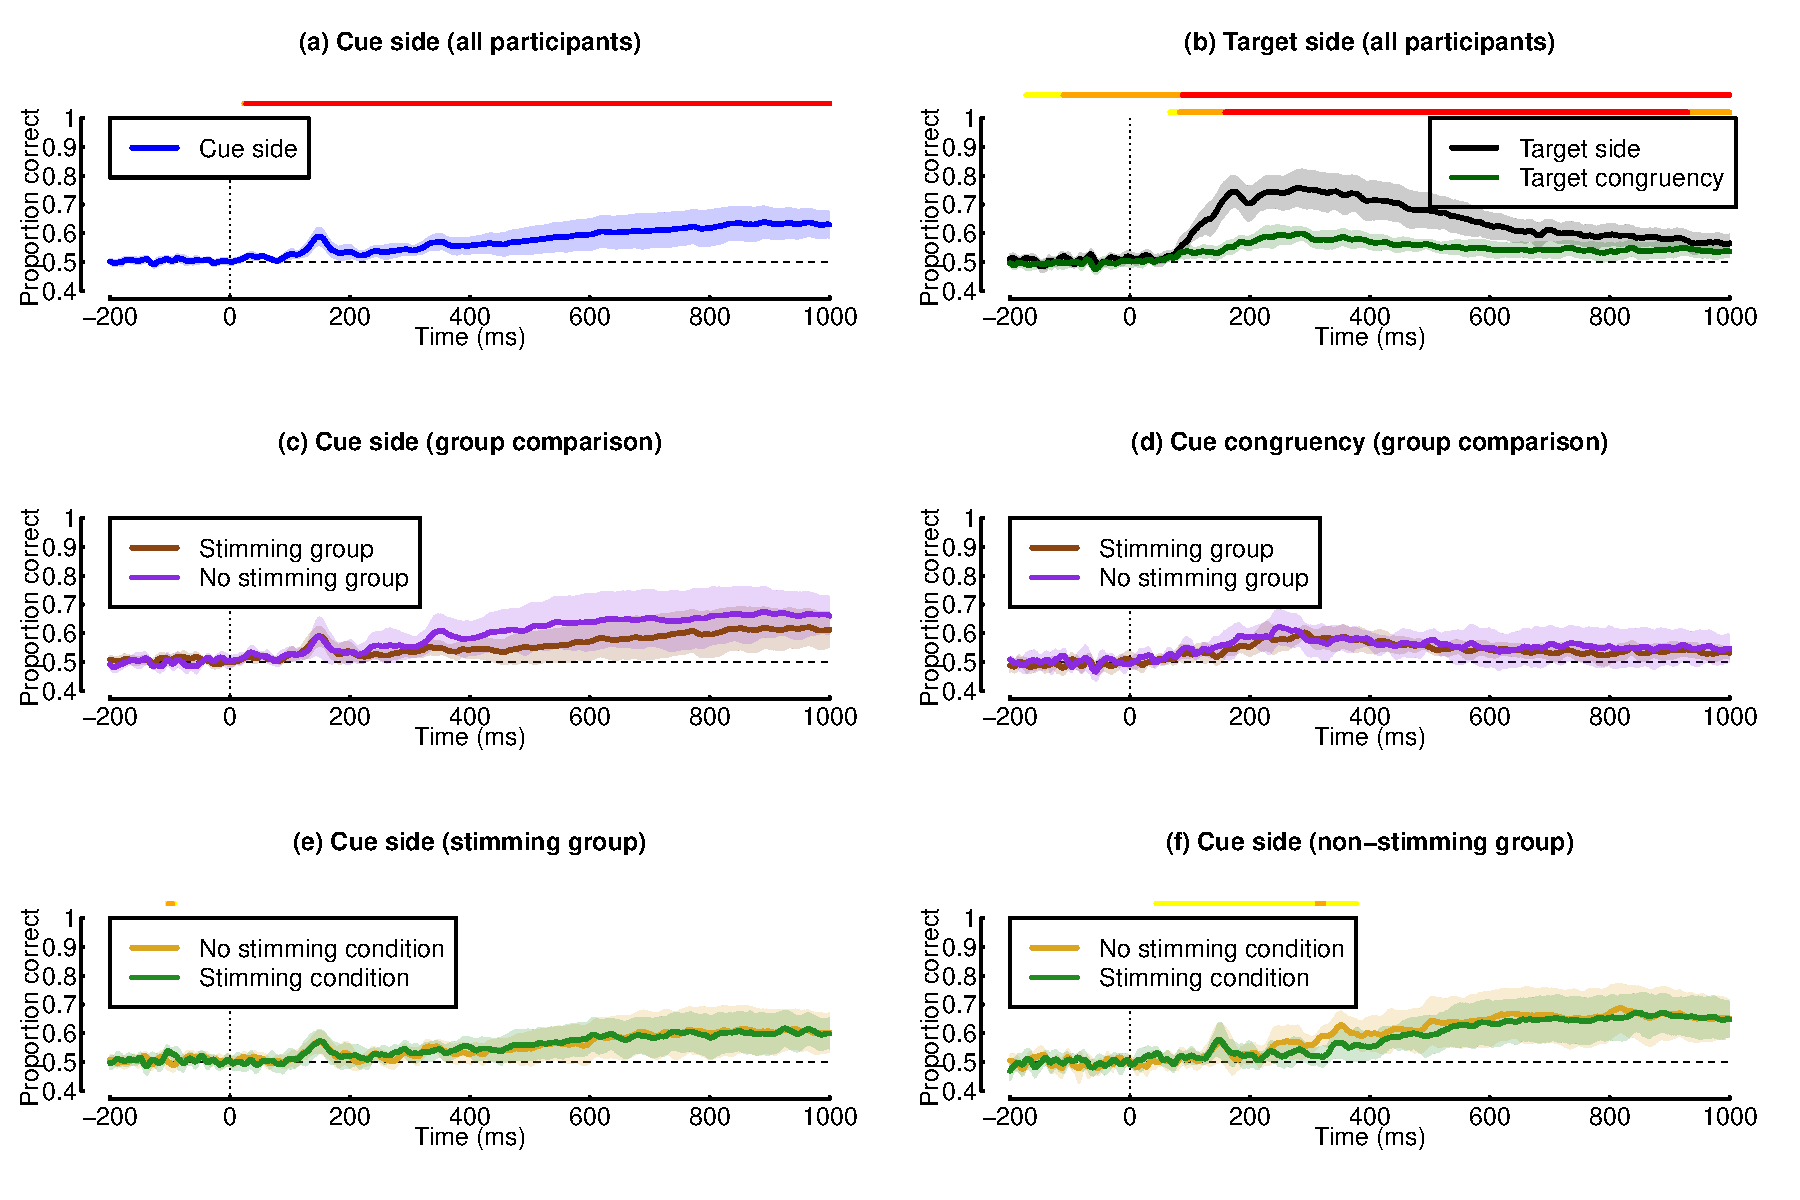
\includegraphics{Figures/Exp2summary.pdf}

}

\caption{\label{fig-Expt2EEG}Summary of EEG data from Experiment 2.
Panel (a) shows decoding accuracy of a pattern classification algorithm
trained on responses to the cue stimulus (Time 0 is the cue onset) for
the full sample of participants (N=22). Panel (b) shows decoding
accuracy for classifying target location (black curve) or cue congruency
(green curve) in response to the target (Time 0 is the target onset),
again for all participants. Panels (c,d) compare decoding between the
stimming (N=14) and non-stimming (N=8) participants for cue side and cue
congruency. Panels (e,f) compare decoding accuracy for cue side within
each group, and between the stimming and no stimming conditions. Shaded
regions in all panels indicate 95\% confidence intervals, and lines
above y=1 indicate Bayes factor scores above 3 (yellow \textgreater3;
orange \textgreater10; red \textgreater30).}

\end{figure}%

We collected eye tracking data for a subset of the participants in
Experiment 2 (16/22; for the remaining participants, the eye tracker was
not able to calibrate successfully). We used these data to check if
participants were able to follow the task instructions and fixate
centrally throughout. The results are summarised in
Figure~\ref{fig-eyepositions}. The grey distributions indicate
horizontal fixation positions at the time of cue onset. For most
participants these are close to the central fixation (0 deg, see
vertical dashed line), though there are some notable consistent offsets
that we attribute to calibration errors (e.g.~P201, P223, P224). The
coloured distributions indicate horizontal fixation positions at the
time of target onset, following either a leftward (blue) or rightward
(red) pointing cue. The majority of participants were able to follow the
instructions and fixated centrally for both of these conditions, showing
no systematic differences. One participant (P214) clearly made eye
movements in the cued direction on most trials, and some participants
(e.g.~P209, P216, P218) showed evidence of sometimes making such eye
movements. At a group level, there was a marginally significant
difference between the mean horizontal positions for left vs right cues
(\(t\) = 2.15, \(p\) \textless{} 0.05), but the overall evidence was not
compelling (\(log_{10}BF_{10}\) = 0.19). We therefore conclude that in
general participants were able to follow instructions appropriately, and
that eye movements are unlikely to be responsible for the EEG effects of
cueing.

\begin{figure}

\centering{

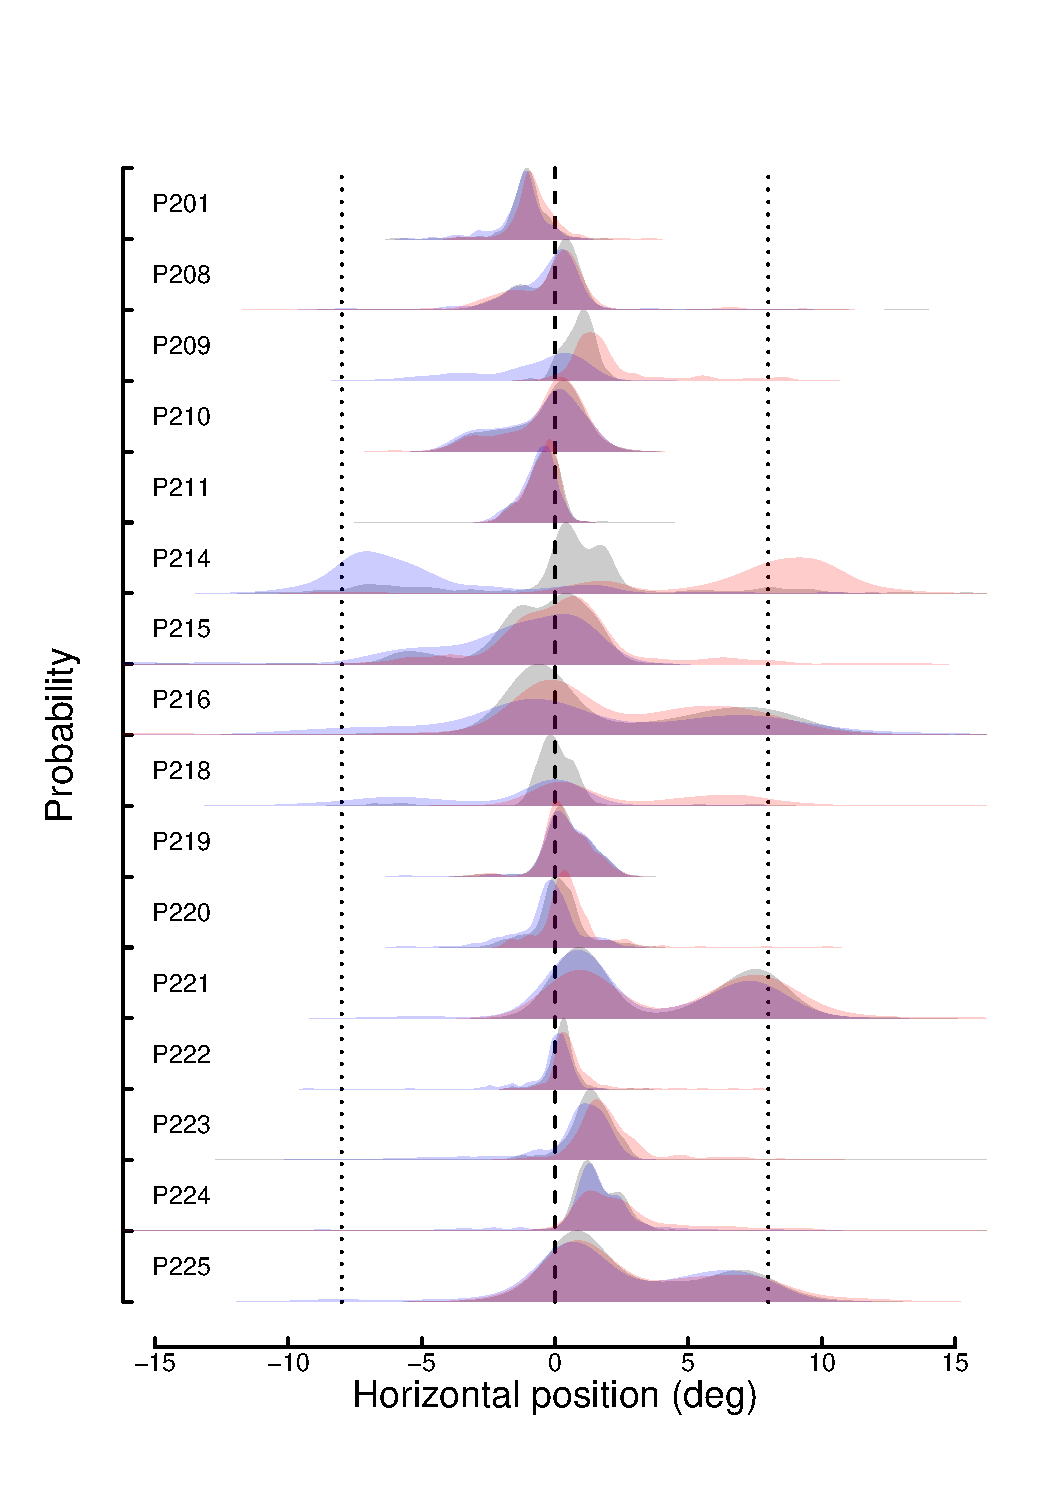
\includegraphics[width=0.6\textwidth,height=\textheight]{Figures/eyepositions.pdf}

}

\caption{\label{fig-eyepositions}Distributions of horizontal eye
positions for 16 participants during Experiment 2. Grey distributions
represent eye positions at cue onset. Coloured distributions represent
eye positions at target onset following a leftward pointing cue (blue)
or a rightward pointing cue (red). Dotted vertical lines indicate the
target locations (±8 degrees).}

\end{figure}%

\section{Discussion}\label{discussion}

Overall, our results from Experiment 1 support the assertion that EEG
data can be used as a metric of attentional deployment {[}13{]}. The
classifier was able to differentiate both cue and target side from EEG
recordings in Experiment 1, indicating we have recorded a neural
correlate of attentional deployment, and that it is possible for a
machine learning classifier to determine the direction of spatial
attention using EEG signals. Extending this method in Experiment 2 by
including the stimming manipulation suggested that stimming does not
have a detrimental effect on attentional deployment, with our only
negative impact of stimming being on reaction times. We will now discuss
these results in greater detail, with a focus on the implications for
research into stimming in the context of the neurodiversity movement.

Behavioural data from Experiment 1 revealed a significant effect of
congruency on both accuracy and reaction time, a typical Posner cueing
effect wherein higher accuracy and shorter reaction times are associated
with congruent relative to incongruent conditions {[}13,14{]}.
Experiment 1 further involved testing the classifier, which revealed
that cue side was reliably decoded from 300ms post-stimulus onset
onwards, reaching an accuracy level of 69\%, and target side was
reliably decoded from much earlier (100ms post-stimulus onset) and
reached 89\% accuracy. This sufficiently validated the use of the
measure in Experiment 2 and supported prior research using similar
techniques {[}13{]}.

Experiment 2 replicated this methodology with the addition of the
stimming manipulation. Additionally, eye position data were recorded
where possible, allowing us to confirm that in the majority of cases
participants understood and followed the instructions, keeping their
eyes fixated on the centre of the screen, and did not overtly move them
following the cue. This confirms that the neural correlates we measured
do not reflect eye movements, suggesting they are instead a genuine
representation of the deployment of spatial attention.

Analysis of the behavioural data revealed no significant effect of
either stimming or congruency on accuracy. The effect of congruency on
accuracy in Posner cueing tasks is robust {[}13,14{]} and our version of
the task generated this effect in Experiment 1, suggesting an external
factor resulted in this difference in Experiment 2. For example, the
environmental conditions under which participants completed the
experiment were quite different, as data for Experiment 1 were collected
over the winter, while Experiment 2 was conducted in the summer, when
the laboratory was very warm, potentially reducing participants' ability
to focus on the task. Accuracy was lower overall for Experiment 2 than
Experiment 1; participants in Experiment 1 averaged 96\% correct for
congruent trials and 93\% correct for incongruent trials, while
participants in Experiment 2 averaged 86\% correct for both congruent
trials and incongruent trials. Difficulties resulting from external
factors such as temperature and general comfort may have influenced the
participants' ability to attend to the experiment to the point where
differences in accuracy became non-significant. Our finding that
stimming had no effect on accuracy would therefore need to be validated
through future replication; should it hold, it is an important one, as
it suggests that stimming does not have a negative impact on
individuals' performance, countering the notion that stimming behaviours
are detrimental and should be targeted through interventions {[}e.g.,
30,45{]}. These findings do not fully align with self-reports from
autistic individuals, however, who report that stimming benefits
attention {[}6{]}; accuracy was no greater in stimming conditions than
non-stimming conditions. This may result from the proportion of our
participants with autism being very small, so future research should aim
to further investigate this in a larger sample. It has been suggested
that stimming acts are a compensatory mechanism {[}6{]} for the
previously discussed attention problems associated with autism {[}5{]},
so there is a possibility that positive effects of stimming are only
seen in these individuals, which warrants further investigation.

Reaction times for participants in Experiment 2 were also longer than
for those in Experiment 1, again suggesting the participants experienced
greater difficulty when completing the task under the external
conditions of the second experiment. In Experiment 1, the average
reaction time was 484ms for congruent trials and 535ms for incongruent
trials, while in Experiment 2, the average reaction time was 557ms/611ms
for congruent trials and 627/654ms for incongruent trials (for
non-stimming/stimming conditions, respectively). However, analysis of
the reaction time data did reveal a typical Posner cueing effect in
regard to congruency: congruent trials were associated with shorter
reaction times. Analysis also suggested a negative effect of stimming on
reaction times, with reaction times being significantly slower when
participants were stimming. Given the lack of impact observed on
accuracy (and on EEG decoding, discussed next) it is likely this finding
relates to stimming interfering with the participants' ability to
complete the task (they were required to respond to stimuli with buttons
on the keyboard while moving their other hand) rather than stimming
being inherently distracting. Participants had to use one hand to stim
while simultaneously responding to stimuli presented on the screen with
the other hand - the incompatibility of the movements being performed
simultaneously may therefore have caused, or contributed to, the
increase in reaction times recorded. Future research into this
phenomenon should modify the task to ensure stimming behaviours are
compatible. Klier and Harris {[}46{]}, for example, used a learning task
where children learnt behaviours either compatible or incompatible with
stimming and found stimming itself did not have a detrimental effect on
the ability to learn. A replication of this study could use a task in
which participants respond verbally, for example, to limit the effect of
incompatible movements. When we further divided participants into those
who reported that they stim in their everyday lives and those who
reported that they did not, we found the pattern only persisted in the
former group; this may be due to the much smaller size of the latter
group, as for the former group the Bayes factor and effect size were
smaller for the effect of stimming than the effect of congruency,
suggesting the relationship between stimming and reaction time is weaker
than between congruency and reaction time. In a larger group of
individuals who do not typically engage in stimming, this relationship
might persist. Future research should aim to recruit larger sample sizes
for various neurotypes and everyday stimming behaviours. It should also
aim to adapt tasks so that there is no potential for the physical motion
of stimming to interfere with the physical motion of completing a task,
allowing the pure effects of stimming to be investigated.

Classifier accuracy in Experiment 2 was lower overall than in Experiment
1, which was not unexpected given the smaller sample size and the fact
that participants in Experiment 2 were moving, potentially introducing
extra noise to the EEG signal. Within Experiment 2, classifier accuracy
was largely similar between individuals who reported typically stimming
and those who did not, validating comparisons between the groups based
on classifier accuracy.

A decrease in classifier accuracy during stimming was observed
exclusively in the group who reported that they did not typically stim.
The same was not true for the typically stimming group. We consider
classifier accuracy here to be a measure of the strength of an
individual's ability to deploy their spatial attention, as stronger
attentional deployment to the left or right should result in a greater
condition-based difference in neural activity, making it easier for the
classifier to differentiate the direction of their attention. Therefore,
this suggests an individual's ability to deploy their spatial attention
is only reduced when they are asked to stim if they do not typically
engage in the behaviour, contesting the notion that stimming is an
inherently harmful behaviour. Further, it may give insight into where
this concept originated; for individuals who do not typically stim, it
appears to have negative consequences for their attentional abilities,
which may lead them to assume that the same is true for everyone (which
our evidence suggests is not the case). For individuals who typically
engage in stimming behaviours, there does not appear to be an impact of
stimming or not stimming on their attentional deployment, indicating
that the behaviour is not detrimental; greater inclusion of neurodiverse
individuals may allow for observation of a positive effect, as stimming
has been proposed as a compensatory mechanism {[}6{]}.

It has long been claimed that stimming behaviours interrupt attention
and learning, which has been used to justify therapies aiming to reduce
these behaviours {[}e.g., 45{]}. Our investigation contests this view,
given our lack of evidence to suggest a negative impact of stimming on
attention. The evidence often used to support this view of stimming
behaviours falls foul to a host of methodological issues, such as
incredibly small groups of participants {[}47{]}, stopping children
stimming entirely during the learning phase {[}48{]}, or not attempting
to prevent stimming behaviours at all {[}49{]}, thereby providing no
real evidence for whether or not stimming affects learning abilities, or
whether reducing them would have a beneficial impact. Indeed,
self-reports from autistic individuals that the behaviours benefit their
attention may mean this view is leading autism interventions in entirely
the wrong direction when it comes to improving the quality of life of
autistic individuals. Interventions that aim to reduce stimming are
worryingly widespread, given their weak research base. Behavioural
approaches, particularly common in North America {[}50{]}, frequently
target these behaviours {[}e.g., 6,51{]}. Future research should attempt
to take a similar approach to ours, investigating and allowing for the
potential that stimming behaviours may have positive effects, or even no
effect at all, to ensure we capture the full picture of stimming and its
potential functions before encouraging interventions that target the
behaviour. One factor that future research should take into
consideration is that in our investigation, we directed participants to
stim or refrain from stimming at certain times. It is unclear whether
there is a subjective difference in stimming when it is genuinely
self-generated compared to when it is externally prompted. Considering
that stimming is believed to address certain internal needs, stimming
when externally prompted (i.e., not in direct response to these needs)
may not generate an effect, because the individual doesn't feel the need
to self-regulate through stimming. This could explain the lack of a
positive effect of stimming that we identified here, if only the truly
self-generated form of stimming produces attentional effects, or any
effects at all. A careful balance needs to be struck between controlling
experimental conditions and ensuring stimming behaviours are authentic
to best understand them. Future research could benefit from a more
naturalistic design, in which participants complete a task while
stimming when it feels natural to them, with researchers recording start
and end times of stimming periods to create stimming and non-stimming
conditions. Likely the ideal method of dealing with this potential
conflict is for researchers across the field to conduct investigations
into stimming in a number of different ways, exploiting the strengths
and weaknesses of various methodologies to obtain a full picture of
stimming. It would also be beneficial to ask individuals who stim
directly about whether or not they believe externally prompted stimming
benefits them in the same way as self-directed stimming.

Another limitation of our investigation was our use of a binary
self-report relating to whether participants typically engaged in
stimming or not. If one were available, it would be beneficial to use a
self-report scale designed to measure an individual's stimming
behaviours. However, at present, the available scales are not
appropriate for this use. The two scales we identified were the
Stereotyped Behaviour Scale (SBS; {[}52{]}) and a sub-section of the
Aberrant Behaviour Checklist (ABC; {[}53{]}) - both scales require an
observer to rate an individual's behaviours, rather than being a
self-report scale, making them unsuitable for use in this context.
Further, the ABC has been criticized for subjective and unacceptable
items- for example using condescending language such as `tantrums' or
describing individuals as `whiny' {[}54{]}. To facilitate further
investigations into stimming it would be beneficial to develop an
appropriate self-report scale, as those currently available are not
suited for this purpose.

Our investigation intended to lay the groundwork for an investigation
into whether stimming behaviours in autism have the same underlying
functions and mechanisms as fidgeting in ADHD. Given our limited sample
size of participants with either disorder, we have not gathered
sufficient evidence to suggest whether or not this is the case. However,
we believe this route is a promising one for investigation under the
framework of the transdiagnostic approach, especially given that there
are overlaps in the benefits of stimming and fidgeting as reported by
individuals with autism and ADHD. Kapp et al. {[}6{]} reported autistic
individuals stated stimming benefitted their ability to focus, while
Canela et al. {[}55{]} similarly reported that individuals with ADHD
stated fidgeting aided in their productivity and concentration.
Similarities have been identified in stimming across ASD and ADHD, with
notable differences including the frequency and complexity of the
movements {[}56{]}. A greater understanding of this behaviour across
conditions may further our understanding of the similarities between
autism and ADHD, a pressing research interest given the high comorbidity
of the two conditions, with the current and lifetime prevalence rates of
ADHD in the autistic population being estimated at 38.5\% and 40.2\%
respectively {[}57{]}.

Future research should additionally pursue other avenues of exploration
into the potential benefits of stimming. In this case, we focused on
attention, given that this is a commonly reported area in which stimming
generates benefits in individuals with autism {[}6{]} and there is
crossover with fidgeting in ADHD, which is also reported to benefit
attention {[}55{]}. However, autistic individuals report a number of
other benefits of stimming, for example emotional regulation
{[}6,7,9,10{]}. In order to obtain a full picture of the mechanisms and
functions of stimming, to fully understand the behaviour and thus inform
interventions which aim to reduce the behaviour, future research should
investigate all reported avenues in which stimming may benefit.

Given that our investigation did not uncover a positive effect of
stimming on attention, it could be suggested that interventions aiming
to reduce stimming behaviours are not causing harm. Often these
interventions are additionally justified on the basis that children who
stim may be socially excluded or bullied as a result of their stimming
behaviours {[}e.g., 58{]}, and engaging in these behaviours can increase
the likelihood of autistic children experiencing bullying {[}59{]},
which is a serious problem. However, even if we assume stimming has no
positive effect (despite self-reports from autistic individuals saying
it does), efforts may be better focused on educating an autistic child's
neurotypical teachers and peers on autism and stimming, cracking down on
bullying, and teaching autistic children how to handle bullying. It has
been demonstrated that describing and explaining autistic behaviours to
children can improve their attitudes towards an autistic child {[}60{]},
and a recent intervention teaching autistic children how to stand up to
bullies achieved a reasonable level of success {[}59{]}. Autistic
children may experience bullying as a result of a wide variety of their
autistic traits {[}61{]}; surely, then, the best approach is to address
the bullying, rather than encouraging autistic children to alter a wide
variety of their own behaviours to avoid it. Particularly in the case of
stimming, autistic adults protest against the elimination of these
behaviours {[}6{]}, and they have been posited as a significant feature
of autistic culture and identity {[}10,36,62{]}. There is also a growing
shift in approaches to teaching autistic children, with new
encouragement of accommodating and integrating stimming into the
classroom environment {[}e.g., 63{]}. Even though we have been unable to
demonstrate in a controlled setting that these behaviours have benefits,
it is important to listen to the community we aim to help and respect
their wishes. This is particularly relevant in the context of the
growing movement for acceptance of neurodiversity, and the push for
inclusion of autistic perspectives in research, as stimming is a
sensitive topic given historical attitudes and current social stigma
surrounding it.

In summary, our results do not support prior literature suggesting
stimming is a behaviour with negative consequences for attention.
Rather, we find that in individuals who typically engage in stimming
behaviours there is no particular detriment associated with doing so
(excluding delayed reaction times, which potentially are an artefact of
the experimental design). Negative impacts of stimming on attentional
deployment were identified in individuals who do not typically engage in
stimming behaviours, which may help explain why the perception has
previously been that the behaviours are detrimental. This research had a
predominantly neurotypical sample, and as such it is vital for future
research to include a greater sample of autistic individuals to
investigate whether stimming functions in the same way for this group as
it appears to for neurotypicals who stim. Furthermore, the inclusion of
a greater sample of individuals with ADHD may help uncover whether the
fidgeting behaviours seen in ADHD may be similar to, or the same as,
autistic stimming. Future research should also aim to investigate the
potential benefits of stimming in a wider range of areas, given that
individuals with autism also report benefits to emotional regulation
{[}6{]} in addition to attention.

\section{Declarations}\label{declarations}

\subsection{Competing interests}\label{competing-interests}

The authors have declared that no competing interests exist.

\subsection{Data availability
statement}\label{data-availability-statement}

Raw data, processed data, and analysis scripts are freely available
through the project repository at: http://doi.org/10.17605/OSF.IO/YUHZ4.

\subsection{Author contributions}\label{author-contributions}

CS: conceived the study, collected the data, performed the analysis,
wrote the paper.

DHB: conceived the study, contributed data, performed the analysis,
wrote the paper.

\section*{References}\label{references}
\addcontentsline{toc}{section}{References}

\phantomsection\label{refs}
\begin{CSLReferences}{0}{1}
\bibitem[\citeproctext]{ref-Knudsen2007}
\CSLLeftMargin{1. }%
\CSLRightInline{Knudsen EI. Fundamental components of attention. Annu
Rev Neurosci. 2007;30: 57--78.
doi:\href{https://doi.org/10.1146/annurev.neuro.30.051606.094256}{10.1146/annurev.neuro.30.051606.094256}}

\bibitem[\citeproctext]{ref-Hopfinger2000}
\CSLLeftMargin{2. }%
\CSLRightInline{Hopfinger JB, Buonocore MH, Mangun GR. The neural
mechanisms of top-down attentional control. Nat Neurosci. 2000;3:
284--91. doi:\href{https://doi.org/10.1038/72999}{10.1038/72999}}

\bibitem[\citeproctext]{ref-Rueda2011}
\CSLLeftMargin{3. }%
\CSLRightInline{Rueda MR, Posner MI, Rothbart MK. 15: Attentional
control and self-regulation. 2nd ed. In: Vohs KD, Baumeister RF,
editors. Handbook of self-regulation. 2nd ed. Guilford Press; 2011. pp.
284--299. }

\bibitem[\citeproctext]{ref-Posner1980}
\CSLLeftMargin{4. }%
\CSLRightInline{Posner MI. Orienting of attention. Q J Exp Psychol.
1980;32: 3--25.
doi:\href{https://doi.org/10.1080/00335558008248231}{10.1080/00335558008248231}}

\bibitem[\citeproctext]{ref-Allen2001}
\CSLLeftMargin{5. }%
\CSLRightInline{Allen G, Courchesne E. Attention function and
dysfunction in autism. Front Biosci. 2001;6: D105--19.
doi:\href{https://doi.org/10.2741/allen}{10.2741/allen}}

\bibitem[\citeproctext]{ref-Kapp2019}
\CSLLeftMargin{6. }%
\CSLRightInline{Kapp SK, Steward R, Crane L, Elliott D, Elphick C,
Pellicano E, et al. 'People should be allowed to do what they like':
Autistic adults' views and experiences of stimming. Autism. 2019;23:
1782--1792.
doi:\href{https://doi.org/10.1177/1362361319829628}{10.1177/1362361319829628}}

\bibitem[\citeproctext]{ref-Steward2015}
\CSLLeftMargin{7. }%
\CSLRightInline{Steward R. Repetitive stereotyped behaviour or
{``stimming''}: An online survey of 100 people on the autism spectrum.
INSAR conference; 2015. Available:
\url{https://insar.confex.com/insar/2015/webprogram/Paper20115.html}}

\bibitem[\citeproctext]{ref-Metz2024}
\CSLLeftMargin{8. }%
\CSLRightInline{Metz S. Stimming as a form of autistic aesthetic
experience, neuroqueering landscape. Ought: The Journal of Autistic
Culture. 2024;5.
doi:\href{https://doi.org/10.9707/2833-1508.1165}{10.9707/2833-1508.1165}}

\bibitem[\citeproctext]{ref-Sagar2024}
\CSLLeftMargin{9. }%
\CSLRightInline{Sagar E, Khera SN, Garg N. "I wish they'd just let us
be." experiences of indian autistic individuals around stimming
behaviors at the workplace. Autism Adulthood. 2024;6: 474--484.
doi:\href{https://doi.org/10.1089/aut.2022.0096}{10.1089/aut.2022.0096}}

\bibitem[\citeproctext]{ref-Petty2024}
\CSLLeftMargin{10. }%
\CSLRightInline{Petty S, Ellis A. The meaning of autistic movements.
Autism. 2024;28: 3015--3020.
doi:\href{https://doi.org/10.1177/13623613241262151}{10.1177/13623613241262151}}

\bibitem[\citeproctext]{ref-McCarty2021}
\CSLLeftMargin{11. }%
\CSLRightInline{McCarty MJ, Brumback AC. Rethinking stereotypies in
autism. Seminars in Pediatric Neurology. 2021;38: 100897.
doi:\url{https://doi.org/10.1016/j.spen.2021.100897}}

\bibitem[\citeproctext]{ref-Leblanc2008}
\CSLLeftMargin{12. }%
\CSLRightInline{Leblanc E, Prime DJ, Jolicoeur P. Tracking the location
of visuospatial attention in a contingent capture paradigm. J Cogn
Neurosci. 2008;20: 657--71.
doi:\href{https://doi.org/10.1162/jocn.2008.20051}{10.1162/jocn.2008.20051}}

\bibitem[\citeproctext]{ref-Thiery2016}
\CSLLeftMargin{13. }%
\CSLRightInline{Thiery T, Lajnef T, Jerbi K, Arguin M, Aubin M,
Jolicoeur P. Decoding the locus of covert visuospatial attention from
EEG signals. PLoS One. 2016;11: e0160304.
doi:\href{https://doi.org/10.1371/journal.pone.0160304}{10.1371/journal.pone.0160304}}

\bibitem[\citeproctext]{ref-Posner1978}
\CSLLeftMargin{14. }%
\CSLRightInline{Posner MI. Chronometric explorations of mind. Lawrence
Erlbaum; 1978. }

\bibitem[\citeproctext]{ref-Landau2007}
\CSLLeftMargin{15. }%
\CSLRightInline{Landau AN, Esterman M, Robertson LC, Bentin S,
Prinzmetal W. Different effects of voluntary and involuntary attention
on EEG activity in the gamma band. Journal of Neuroscience. 2007;27:
11986--11990. }

\bibitem[\citeproctext]{ref-Capotosto2012}
\CSLLeftMargin{16. }%
\CSLRightInline{Capotosto P, Corbetta M, Romani GL, Babiloni C.
Electrophysiological correlates of stimulus-driven reorienting deficits
after interference with right parietal cortex during a spatial attention
task: A TMS-EEG study. J Cogn Neurosci. 2012;24: 2363--71.
doi:\href{https://doi.org/10.1162/jocn_a_00287}{10.1162/jocn\_a\_00287}}

\bibitem[\citeproctext]{ref-Vossel2009}
\CSLLeftMargin{17. }%
\CSLRightInline{Vossel S, Weidner R, Thiel CM, Fink GR. What is "odd" in
posner's location-cueing paradigm? Neural responses to unexpected
location and feature changes compared. J Cogn Neurosci. 2009;21: 30--41.
doi:\href{https://doi.org/10.1162/jocn.2009.21003}{10.1162/jocn.2009.21003}}

\bibitem[\citeproctext]{ref-Peelen2004}
\CSLLeftMargin{18. }%
\CSLRightInline{Peelen MV, Heslenfeld DJ, Theeuwes J. Endogenous and
exogenous attention shifts are mediated by the same large-scale neural
network. NeuroImage. 2004;22: 822--830.
doi:\url{https://doi.org/10.1016/j.neuroimage.2004.01.044}}

\bibitem[\citeproctext]{ref-Fitzgerald2015}
\CSLLeftMargin{19. }%
\CSLRightInline{Fitzgerald J, Johnson K, Kehoe E, Bokde ALW, Garavan H,
Gallagher L, et al. Disrupted functional connectivity in dorsal and
ventral attention networks during attention orienting in autism spectrum
disorders. Autism Res. 2015;8: 136--52.
doi:\href{https://doi.org/10.1002/aur.1430}{10.1002/aur.1430}}

\bibitem[\citeproctext]{ref-Dupuis2022}
\CSLLeftMargin{20. }%
\CSLRightInline{Dupuis A, Mudiyanselage P, Burton CL, Arnold PD, Crosbie
J, Schachar RJ. Hyperfocus or flow? Attentional strengths in autism
spectrum disorder. Front Psychiatry. 2022;13: 886692.
doi:\href{https://doi.org/10.3389/fpsyt.2022.886692}{10.3389/fpsyt.2022.886692}}

\bibitem[\citeproctext]{ref-Hupfeld2019}
\CSLLeftMargin{21. }%
\CSLRightInline{Hupfeld KE, Abagis TR, Shah P. Living "in the zone":
Hyperfocus in adult ADHD. Atten Defic Hyperact Disord. 2019;11:
191--208.
doi:\href{https://doi.org/10.1007/s12402-018-0272-y}{10.1007/s12402-018-0272-y}}

\bibitem[\citeproctext]{ref-Astle2022}
\CSLLeftMargin{22. }%
\CSLRightInline{Astle DE, Holmes J, Kievit R, Gathercole SE. Annual
research review: The transdiagnostic revolution in neurodevelopmental
disorders. J Child Psychol Psychiatry. 2022;63: 397--417.
doi:\href{https://doi.org/10.1111/jcpp.13481}{10.1111/jcpp.13481}}

\bibitem[\citeproctext]{ref-Zhang2022}
\CSLLeftMargin{23. }%
\CSLRightInline{Zhang M, Huang Y, Jiao J, Yuan D, Hu X, Yang P, et al.
Transdiagnostic symptom subtypes across autism spectrum disorders and
attention deficit hyperactivity disorder: Validated by measures of
neurocognition and structural connectivity. BMC Psychiatry. 2022;22:
102.
doi:\href{https://doi.org/10.1186/s12888-022-03734-4}{10.1186/s12888-022-03734-4}}

\bibitem[\citeproctext]{ref-Chadehumbe2018}
\CSLLeftMargin{24. }%
\CSLRightInline{Chadehumbe M. A comprehensive review of motor
stereotypies in children. Current Pediatrics Reports. 2018;6: 30--33.
doi:\href{https://doi.org/10.1007/s40124-018-0153-z}{10.1007/s40124-018-0153-z}}

\bibitem[\citeproctext]{ref-Mackenzie2018}
\CSLLeftMargin{25. }%
\CSLRightInline{Mackenzie K. Stereotypic movement disorders. Seminars in
Pediatric Neurology. 2018;25: 19--24.
doi:\url{https://doi.org/10.1016/j.spen.2017.12.004}}

\bibitem[\citeproctext]{ref-Tan1997}
\CSLLeftMargin{26. }%
\CSLRightInline{Tan A, Salgado M, Fahn S. The characterization and
outcome of stereotypical movements in nonautistic children. Mov Disord.
1997;12: 47--52.
doi:\href{https://doi.org/10.1002/mds.870120109}{10.1002/mds.870120109}}

\bibitem[\citeproctext]{ref-Charlop1983}
\CSLLeftMargin{27. }%
\CSLRightInline{Charlop MH. The effects of echolalia on acquisition and
generalization of receptive labeling in autistic children. J Appl Behav
Anal. 1983;16: 111--26.
doi:\href{https://doi.org/10.1901/jaba.1983.16-111}{10.1901/jaba.1983.16-111}}

\bibitem[\citeproctext]{ref-Pruccoli2021}
\CSLLeftMargin{28. }%
\CSLRightInline{Pruccoli J, Spadoni C, Orsenigo A, Parmeggiani A. Should
echolalia be considered a phonic stereotypy? A narrative review. Brain
Sci. 2021;11.
doi:\href{https://doi.org/10.3390/brainsci11070862}{10.3390/brainsci11070862}}

\bibitem[\citeproctext]{ref-Prizant1981}
\CSLLeftMargin{29. }%
\CSLRightInline{Prizant BM, Duchan JF. The functions of immediate
echolalia in autistic children. J Speech Hear Disord. 1981;46: 241--9.
doi:\href{https://doi.org/10.1044/jshd.4603.241}{10.1044/jshd.4603.241}}

\bibitem[\citeproctext]{ref-FertelDaly2001}
\CSLLeftMargin{30. }%
\CSLRightInline{Fertel-Daly D, Bedell G, Hinojosa J. Effects of a
weighted vest on attention to task and self-stimulatory behaviors in
preschoolers with pervasive developmental disorders. The American
Journal of Occupational Therapy. 2001;55: 629–640.
doi:\href{https://doi.org/10.5014/ajot.55.6.629}{10.5014/ajot.55.6.629}}

\bibitem[\citeproctext]{ref-Milne2009}
\CSLLeftMargin{31. }%
\CSLRightInline{Milne E, Scope A, Pascalis O, Buckley D, Makeig S.
Independent component analysis reveals atypical electroencephalographic
activity during visual perception in individuals with autism. Biol
Psychiatry. 2009;65: 22--30.
doi:\href{https://doi.org/10.1016/j.biopsych.2008.07.017}{10.1016/j.biopsych.2008.07.017}}

\bibitem[\citeproctext]{ref-Snijders2013}
\CSLLeftMargin{32. }%
\CSLRightInline{Snijders TM, Milivojevic B, Kemner C. Atypical
excitation-inhibition balance in autism captured by the gamma response
to contextual modulation. Neuroimage Clin. 2013;3: 65--72.
doi:\href{https://doi.org/10.1016/j.nicl.2013.06.015}{10.1016/j.nicl.2013.06.015}}

\bibitem[\citeproctext]{ref-Murphy2017}
\CSLLeftMargin{33. }%
\CSLRightInline{Murphy E, Benı́tez-Burraco A. Language deficits in
schizophrenia and autism as related oscillatory connectomopathies: An
evolutionary account. Neurosci Biobehav Rev. 2017;83: 742--764.
doi:\href{https://doi.org/10.1016/j.neubiorev.2016.07.029}{10.1016/j.neubiorev.2016.07.029}}

\bibitem[\citeproctext]{ref-Wang2013}
\CSLLeftMargin{34. }%
\CSLRightInline{Wang J, Barstein J, Ethridge LE, Mosconi MW, Takarae Y,
Sweeney JA. Resting state EEG abnormalities in autism spectrum
disorders. J Neurodev Disord. 2013;5: 24.
doi:\href{https://doi.org/10.1186/1866-1955-5-24}{10.1186/1866-1955-5-24}}

\bibitem[\citeproctext]{ref-Berman2015}
\CSLLeftMargin{35. }%
\CSLRightInline{Berman JI, Liu S, Bloy L, Blaskey L, Roberts TPL, Edgar
JC. Alpha-to-gamma phase-amplitude coupling methods and application to
autism spectrum disorder. Brain Connect. 2015;5: 80--90.
doi:\href{https://doi.org/10.1089/brain.2014.0242}{10.1089/brain.2014.0242}}

\bibitem[\citeproctext]{ref-Morris2025}
\CSLLeftMargin{36. }%
\CSLRightInline{Morris IF, Sykes JR, Paulus ER, Dameh A, Razzaque A,
Esch LV, et al. Beyond self-regulation: Autistic experiences and
perceptions of stimming. Neurodiversity. 2025;3.
doi:\href{https://doi.org/10.1177/27546330241311096}{10.1177/27546330241311096}}

\bibitem[\citeproctext]{ref-Chen2024}
\CSLLeftMargin{37. }%
\CSLRightInline{Chen RSY. Bridging the gap: Fostering interactive
stimming between non-speaking autistic children and their parents. Front
Integr Neurosci. 2024;18: 1374882.
doi:\href{https://doi.org/10.3389/fnint.2024.1374882}{10.3389/fnint.2024.1374882}}

\bibitem[\citeproctext]{ref-Kleiner2007}
\CSLLeftMargin{38. }%
\CSLRightInline{Kleiner M, Brainard DH, Pelli DG. What's new in
psychtoolbox-3? Perception. 2007;36S: 14. }

\bibitem[\citeproctext]{ref-Brainard1997}
\CSLLeftMargin{39. }%
\CSLRightInline{Brainard DH.
\href{https://www.ncbi.nlm.nih.gov/pubmed/9176952}{The psychophysics
toolbox}. Spat Vis. 1997;10: 433--6. }

\bibitem[\citeproctext]{ref-Pelli1997}
\CSLLeftMargin{40. }%
\CSLRightInline{Pelli DG.
\href{https://www.ncbi.nlm.nih.gov/pubmed/9176953}{The VideoToolbox
software for visual psychophysics: Transforming numbers into movies}.
Spat Vis. 1997;10: 437--42. }

\bibitem[\citeproctext]{ref-Tottenham2009}
\CSLLeftMargin{41. }%
\CSLRightInline{Tottenham N, Tanaka JW, Leon AC, McCarry T, Nurse M,
Hare TA, et al. The NimStim set of facial expressions: Judgments from
untrained research participants. Psychiatry Res. 2009;168: 242--9.
doi:\href{https://doi.org/10.1016/j.psychres.2008.05.006}{10.1016/j.psychres.2008.05.006}}

\bibitem[\citeproctext]{ref-Delorme2004}
\CSLLeftMargin{42. }%
\CSLRightInline{Delorme A, Makeig S. {EEGLAB}: An open source toolbox
for analysis of single-trial {EEG} dynamics including independent
component analysis. J Neurosci Methods. 2004;134: 9--21.
doi:\href{https://doi.org/10.1016/j.jneumeth.2003.10.009}{10.1016/j.jneumeth.2003.10.009}}

\bibitem[\citeproctext]{ref-Gramfort2013}
\CSLLeftMargin{43. }%
\CSLRightInline{Gramfort A, Luessi M, Larson E, Engemann DA, Strohmeier
D, Brodbeck C, et al. MEG and EEG data analysis with MNE-python. Front
Neurosci. 2013;7: 267.
doi:\href{https://doi.org/10.3389/fnins.2013.00267}{10.3389/fnins.2013.00267}}

\bibitem[\citeproctext]{ref-Rouder2009}
\CSLLeftMargin{44. }%
\CSLRightInline{Rouder JN, Speckman PL, Sun D, Morey RD, Iverson G.
Bayesian t tests for accepting and rejecting the null hypothesis.
Psychon Bull Rev. 2009;16: 225--37.
doi:\href{https://doi.org/10.3758/PBR.16.2.225}{10.3758/PBR.16.2.225}}

\bibitem[\citeproctext]{ref-Boyd2012}
\CSLLeftMargin{45. }%
\CSLRightInline{Boyd BA, McDonough SG, Bodfish JW. Evidence-based
behavioral interventions for repetitive behaviors in autism. J Autism
Dev Disord. 2012;42: 1236--48.
doi:\href{https://doi.org/10.1007/s10803-011-1284-z}{10.1007/s10803-011-1284-z}}

\bibitem[\citeproctext]{ref-Klier1977}
\CSLLeftMargin{46. }%
\CSLRightInline{Klier J, Harris SL. Self-stimulation and learning in
autistic children: Physical or functional incompatibility? Journal of
Applied Behavior Analysis. 1977;10: 311--311.
doi:\url{https://doi.org/10.1901/jaba.1977.10-311}}

\bibitem[\citeproctext]{ref-Koegel1972}
\CSLLeftMargin{47. }%
\CSLRightInline{Koegel RL, Covert A. The relationship of
self-stimulation to learning in autistic children. J Appl Behav Anal.
1972;5: 381--7.
doi:\href{https://doi.org/10.1901/jaba.1972.5-381}{10.1901/jaba.1972.5-381}}

\bibitem[\citeproctext]{ref-Varni1979}
\CSLLeftMargin{48. }%
\CSLRightInline{Varni JW, Lovaas OI, Koegel RL, Everett NL. An analysis
of observational learning in autistic and normal children. J Abnorm
Child Psychol. 1979;7: 31--43.
doi:\href{https://doi.org/10.1007/BF00924508}{10.1007/BF00924508}}

\bibitem[\citeproctext]{ref-Pierce2001}
\CSLLeftMargin{49. }%
\CSLRightInline{Pierce K, Courchesne E. Evidence for a cerebellar role
in reduced exploration and stereotyped behavior in autism. Biol
Psychiatry. 2001;49: 655--64.
doi:\href{https://doi.org/10.1016/s0006-3223(00)01008-8}{10.1016/s0006-3223(00)01008-8}}

\bibitem[\citeproctext]{ref-Keenan2015}
\CSLLeftMargin{50. }%
\CSLRightInline{Keenan M, Dillenburger K, Röttgers HR, Dounavi K,
Jónsdóttir SL, Moderato P, et al. Autism and ABA: The gulf between north
america and europe. Review Journal of Autism and Developmental
Disorders. 2015;2: 167--183.
doi:\href{https://doi.org/10.1007/s40489-014-0045-2}{10.1007/s40489-014-0045-2}}

\bibitem[\citeproctext]{ref-Raulston2019}
\CSLLeftMargin{51. }%
\CSLRightInline{Raulston TJ, Hansen SG, Machalicek W, McIntyre LL,
Carnett A. Interventions for repetitive behavior in young children with
autism: A survey of behavioral practices. J Autism Dev Disord. 2019;49:
3047--3059.
doi:\href{https://doi.org/10.1007/s10803-019-04023-y}{10.1007/s10803-019-04023-y}}

\bibitem[\citeproctext]{ref-Rojahn2000}
\CSLLeftMargin{52. }%
\CSLRightInline{Rojahn J, Matlock ST, Tassé MJ. The stereotyped behavior
scale: Psychometric properties and norms. Res Dev Disabil. 2000;21:
437--54.
doi:\href{https://doi.org/10.1016/s0891-4222(00)00057-3}{10.1016/s0891-4222(00)00057-3}}

\bibitem[\citeproctext]{ref-Aman1985}
\CSLLeftMargin{53. }%
\CSLRightInline{Aman MG, Singh NN, Stewart AW, Field CJ.
\href{https://www.ncbi.nlm.nih.gov/pubmed/3993694}{The aberrant behavior
checklist: A behavior rating scale for the assessment of treatment
effects}. Am J Ment Defic. 1985;89: 485--91. }

\bibitem[\citeproctext]{ref-Chan2020}
\CSLLeftMargin{54. }%
\CSLRightInline{Chan B, Baker P. An evaluation of the social validity of
the aberrant behavior checklist - community. Tizard Learning Disability
Review. 2020;25: 53--61.
doi:\href{https://doi.org/10.1108/tldr-12-2019-0038}{10.1108/tldr-12-2019-0038}}

\bibitem[\citeproctext]{ref-Canela2017}
\CSLLeftMargin{55. }%
\CSLRightInline{Canela C, Buadze A, Dube A, Eich D, Liebrenz M. Skills
and compensation strategies in adult ADHD - a qualitative study. PLoS
One. 2017;12: e0184964.
doi:\href{https://doi.org/10.1371/journal.pone.0184964}{10.1371/journal.pone.0184964}}

\bibitem[\citeproctext]{ref-Oroian2024}
\CSLLeftMargin{56. }%
\CSLRightInline{Oroian BA, Costandache G, Popescu E, Nechita P,
Szalontay A. Comparative analysis of self-stimulatory behaviors in ASD
and ADHD. European Psychiatry. 2024;67: S220–S220.
doi:\href{https://doi.org/10.1192/j.eurpsy.2024.471}{10.1192/j.eurpsy.2024.471}}

\bibitem[\citeproctext]{ref-Rong2021}
\CSLLeftMargin{57. }%
\CSLRightInline{Rong Y, Yang C-J, Jin Y, Wang Y. Prevalence of
attention-deficit/hyperactivity disorder in individuals with autism
spectrum disorder: A meta-analysis. Research in Autism Spectrum
Disorders. 2021;83: 101759.
doi:\url{https://doi.org/10.1016/j.rasd.2021.101759}}

\bibitem[\citeproctext]{ref-Tse2018}
\CSLLeftMargin{58. }%
\CSLRightInline{Tse CYA, Pang CL, Lee PH. Choosing an appropriate
physical exercise to reduce stereotypic behavior in children with autism
spectrum disorders: A non-randomized crossover study. J Autism Dev
Disord. 2018;48: 1666--1672.
doi:\href{https://doi.org/10.1007/s10803-017-3419-3}{10.1007/s10803-017-3419-3}}

\bibitem[\citeproctext]{ref-Rex2018}
\CSLLeftMargin{59. }%
\CSLRightInline{Rex C, Charlop MH, Spector V. Using video modeling as an
anti-bullying intervention for children with autism spectrum disorder. J
Autism Dev Disord. 2018;48: 2701--2713.
doi:\href{https://doi.org/10.1007/s10803-018-3527-8}{10.1007/s10803-018-3527-8}}

\bibitem[\citeproctext]{ref-Campbell2004}
\CSLLeftMargin{60. }%
\CSLRightInline{Campbell JM, Ferguson JE, Herzinger CV, Jackson JN,
Marino CA. Combined descriptive and explanatory information improves
peers' perceptions of autism. Res Dev Disabil. 2004;25: 321--39.
doi:\href{https://doi.org/10.1016/j.ridd.2004.01.005}{10.1016/j.ridd.2004.01.005}}

\bibitem[\citeproctext]{ref-Chen2012}
\CSLLeftMargin{61. }%
\CSLRightInline{Chen P-Y, Schwartz IS. Bullying and victimization
experiences of students with autism spectrum disorders in elementary
schools. Focus on Autism and Other Developmental Disabilities. 2012;27:
200–212.
doi:\href{https://doi.org/10.1177/1088357612459556}{10.1177/1088357612459556}}

\bibitem[\citeproctext]{ref-Felepchuk2021}
\CSLLeftMargin{62. }%
\CSLRightInline{Felepchuk E. Stimming, improvisation, and COVID-19:
(Re)negotiating autistic sensory regulation during a pandemic.
Disability Studies Quarterly. 2021;41.
doi:\href{https://doi.org/10.18061/dsq.v41i3}{10.18061/dsq.v41i3}}

\bibitem[\citeproctext]{ref-Tancredi2024}
\CSLLeftMargin{63. }%
\CSLRightInline{Tancredi S, Abrahamson D. Stimming as thinking: A
critical reevaluation of self-stimulatory behavior as an epistemic
resource for inclusive education. Educational Psychology Review.
2024;36: 75.
doi:\href{https://doi.org/10.1007/s10648-024-09904-y}{10.1007/s10648-024-09904-y}}

\end{CSLReferences}



\end{document}
